\documentclass[twoside]{book}

% Packages required by doxygen
\usepackage{fixltx2e}
\usepackage{calc}
\usepackage{doxygen}
\usepackage[export]{adjustbox} % also loads graphicx
\usepackage{graphicx}
\usepackage[utf8]{inputenc}
\usepackage{makeidx}
\usepackage{multicol}
\usepackage{multirow}
\PassOptionsToPackage{warn}{textcomp}
\usepackage{textcomp}
\usepackage[nointegrals]{wasysym}
\usepackage[table]{xcolor}

% Font selection
\usepackage[T1]{fontenc}
\usepackage[scaled=.90]{helvet}
\usepackage{courier}
\usepackage{amssymb}
\usepackage{sectsty}
\renewcommand{\familydefault}{\sfdefault}
\allsectionsfont{%
  \fontseries{bc}\selectfont%
  \color{darkgray}%
}
\renewcommand{\DoxyLabelFont}{%
  \fontseries{bc}\selectfont%
  \color{darkgray}%
}
\newcommand{\+}{\discretionary{\mbox{\scriptsize$\hookleftarrow$}}{}{}}

% Page & text layout
\usepackage{geometry}
\geometry{%
  a4paper,%
  top=2.5cm,%
  bottom=2.5cm,%
  left=2.5cm,%
  right=2.5cm%
}
\tolerance=750
\hfuzz=15pt
\hbadness=750
\setlength{\emergencystretch}{15pt}
\setlength{\parindent}{0cm}
\setlength{\parskip}{3ex plus 2ex minus 2ex}
\makeatletter
\renewcommand{\paragraph}{%
  \@startsection{paragraph}{4}{0ex}{-1.0ex}{1.0ex}{%
    \normalfont\normalsize\bfseries\SS@parafont%
  }%
}
\renewcommand{\subparagraph}{%
  \@startsection{subparagraph}{5}{0ex}{-1.0ex}{1.0ex}{%
    \normalfont\normalsize\bfseries\SS@subparafont%
  }%
}
\makeatother

% Headers & footers
\usepackage{fancyhdr}
\pagestyle{fancyplain}
\fancyhead[LE]{\fancyplain{}{\bfseries\thepage}}
\fancyhead[CE]{\fancyplain{}{}}
\fancyhead[RE]{\fancyplain{}{\bfseries\leftmark}}
\fancyhead[LO]{\fancyplain{}{\bfseries\rightmark}}
\fancyhead[CO]{\fancyplain{}{}}
\fancyhead[RO]{\fancyplain{}{\bfseries\thepage}}
\fancyfoot[LE]{\fancyplain{}{}}
\fancyfoot[CE]{\fancyplain{}{}}
\fancyfoot[RE]{\fancyplain{}{\bfseries\scriptsize Generated by Doxygen }}
\fancyfoot[LO]{\fancyplain{}{\bfseries\scriptsize Generated by Doxygen }}
\fancyfoot[CO]{\fancyplain{}{}}
\fancyfoot[RO]{\fancyplain{}{}}
\renewcommand{\footrulewidth}{0.4pt}
\renewcommand{\chaptermark}[1]{%
  \markboth{#1}{}%
}
\renewcommand{\sectionmark}[1]{%
  \markright{\thesection\ #1}%
}

% Indices & bibliography
\usepackage{natbib}
\usepackage[titles]{tocloft}
\setcounter{tocdepth}{3}
\setcounter{secnumdepth}{5}
\makeindex

% Hyperlinks (required, but should be loaded last)
\usepackage{ifpdf}
\ifpdf
  \usepackage[pdftex,pagebackref=true]{hyperref}
\else
  \usepackage[ps2pdf,pagebackref=true]{hyperref}
\fi
\hypersetup{%
  colorlinks=true,%
  linkcolor=blue,%
  citecolor=blue,%
  unicode%
}

% Custom commands
\newcommand{\clearemptydoublepage}{%
  \newpage{\pagestyle{empty}\cleardoublepage}%
}

\usepackage{caption}
\captionsetup{labelsep=space,justification=centering,font={bf},singlelinecheck=off,skip=4pt,position=top}

%===== C O N T E N T S =====

\begin{document}

% Titlepage & ToC
\hypersetup{pageanchor=false,
             bookmarksnumbered=true,
             pdfencoding=unicode
            }
\pagenumbering{alph}
\begin{titlepage}
\vspace*{7cm}
\begin{center}%
{\Large libgai }\\
\vspace*{1cm}
{\large Generated by Doxygen 1.8.13}\\
\end{center}
\end{titlepage}
\clearemptydoublepage
\pagenumbering{roman}
\tableofcontents
\clearemptydoublepage
\pagenumbering{arabic}
\hypersetup{pageanchor=true}

%--- Begin generated contents ---
\chapter{libgai documentation}
\label{index}\hypertarget{index}{}\hypertarget{index_intro_sec}{}\section{Introduction}\label{index_intro_sec}
A list of all api\textquotesingle{}s currently available. \begin{DoxyNote}{Note}
None of these are actually done yet. They are working but do not support all features!
\end{DoxyNote}
\tabulinesep=1mm
\begin{longtabu} spread 0pt [c]{*{2}{|X[-1]}|}
\hline
\rowcolor{\tableheadbgcolor}\textbf{ filename }&\textbf{ description  }\\\cline{1-2}
\endfirsthead
\hline
\endfoot
\hline
\rowcolor{\tableheadbgcolor}\textbf{ filename }&\textbf{ description  }\\\cline{1-2}
\endhead
\hyperlink{gai__hotreload_8h}{gai\+\_\+hotreload.\+h} &Tracks when a file change happened to a file ( For windows it only check for filetime write changes. So it will trigger an event when you save the file or replace it with another ) \\\cline{1-2}
\hyperlink{gai__xwindow_8h}{gai\+\_\+xwindow.\+h} &Requests a window for all currently supported platforms. \\\cline{1-2}
\end{longtabu}

\chapter{Todo List}
\label{todo}
\Hypertarget{todo}

\begin{DoxyRefList}
\item[\label{todo__todo000001}%
\Hypertarget{todo__todo000001}%
Class \hyperlink{structgaihr__platform}{gaihr\+\_\+platform} ]Add support for multiple platforms! Currently only windows is supported 
\end{DoxyRefList}
\chapter{File Index}
\section{File List}
Here is a list of all documented files with brief descriptions\+:\begin{DoxyCompactList}
\item\contentsline{section}{{\bfseries doxygen.\+h} }{\pageref{doxygen_8h}}{}
\item\contentsline{section}{\hyperlink{gai_8h}{gai.\+h} \\*Designed as a cross platform single include header file for the most necessary features (window, dynamic array, qsort, network) }{\pageref{gai_8h}}{}
\item\contentsline{section}{{\bfseries gai\+\_\+engine.\+h} }{\pageref{gai__engine_8h}}{}
\end{DoxyCompactList}

\chapter{File Documentation}
\hypertarget{gai__hotreload_8h}{}\section{gai\+\_\+hotreload.\+h File Reference}
\label{gai__hotreload_8h}\index{gai\+\_\+hotreload.\+h@{gai\+\_\+hotreload.\+h}}


Tracks when a file change happened to a file ( For windows it only check for filetime write changes. So it will trigger an event when you save the file or replace it with another )  


{\ttfamily \#include $<$windows.\+h$>$}\newline
{\ttfamily \#include $<$assert.\+h$>$}\newline
Include dependency graph for gai\+\_\+hotreload.\+h\+:\nopagebreak
\begin{figure}[H]
\begin{center}
\leavevmode
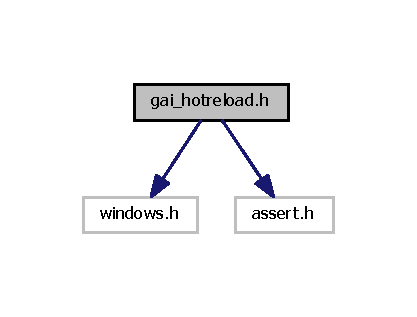
\includegraphics[width=200pt]{gai__hotreload_8h__incl}
\end{center}
\end{figure}
\subsection*{Classes}
\begin{DoxyCompactItemize}
\item 
union \hyperlink{gai__hotreload_8h_uniongaihr__filetime}{gaihr\+\_\+filetime}
\item 
union \hyperlink{gai__hotreload_8h_uniongaihr__platform}{gaihr\+\_\+platform}
\item 
struct \hyperlink{gai__hotreload_8h_structgaihr__platform_1_1gaihr__platform__win32}{gaihr\+\_\+platform\+::gaihr\+\_\+platform\+\_\+win32}
\item 
struct \hyperlink{gai__hotreload_8h_structgaihr__platform_1_1gaihr__platform__linux}{gaihr\+\_\+platform\+::gaihr\+\_\+platform\+\_\+linux}
\item 
struct \hyperlink{gai__hotreload_8h_structgaihr__file}{gaihr\+\_\+file}
\item 
struct \hyperlink{gai__hotreload_8h_structgaihr__filetime_8parts}{gaihr\+\_\+filetime.\+parts}
\end{DoxyCompactItemize}
\subsection*{Macros}
\begin{DoxyCompactItemize}
\item 
\#define \hyperlink{gai__hotreload_8h_a36b03891b740d035afdd1f32e15c91ad}{G\+A\+I\+H\+R\+\_\+\+W\+A\+I\+T\+\_\+\+I\+N\+F\+I\+N\+I\+TE}~-\/1
\item 
\#define \hyperlink{gai__hotreload_8h_a7385b7149ef022fa38140e2b2a540502}{G\+A\+I\+H\+R\+\_\+\+T\+H\+R\+E\+A\+D\+\_\+\+T\+I\+M\+E\+O\+UT}~1000
\item 
\#define \hyperlink{gai__hotreload_8h_ac26b515249679c1f9036430164867ba0}{G\+A\+I\+H\+R\+\_\+\+F\+I\+L\+E\+\_\+\+L\+I\+M\+IT}~64
\item 
\mbox{\Hypertarget{gai__hotreload_8h_a32983003a4e816a8350f01cb22d1b01b}\label{gai__hotreload_8h_a32983003a4e816a8350f01cb22d1b01b}} 
\#define \hyperlink{gai__hotreload_8h_a32983003a4e816a8350f01cb22d1b01b}{G\+A\+I\+H\+R\+\_\+\+A\+PI}~extern
\begin{DoxyCompactList}\small\item\em Define {\bfseries G\+A\+I\+H\+R\+\_\+\+S\+T\+A\+T\+IC} if you want to make functions {\bfseries static} instead of {\bfseries extern} \end{DoxyCompactList}\item 
\#define \hyperlink{gai__hotreload_8h_a11e965cbb3e2af8ed1888b0c6b2777da}{G\+A\+I\+H\+R\+\_\+\+A\+S\+S\+E\+RT}(cond)~assert(cond)
\begin{DoxyCompactList}\small\item\em Define {\bfseries G\+A\+I\+H\+R\+\_\+\+A\+S\+S\+E\+RT} before including this file to {\bfseries disable} assertions. \end{DoxyCompactList}\item 
\#define \hyperlink{gai__hotreload_8h_a6f8c5bfe220445bbbb8e1c9ef176838a}{G\+A\+I\+H\+R\+\_\+\+C\+A\+L\+L\+B\+A\+CK}(name)~void name(\hyperlink{gai__hotreload_8h_structgaihr__file}{gaihr\+\_\+file} $\ast$file)
\begin{DoxyCompactList}\small\item\em Callback function macro which will generate a function as specified by \hyperlink{gai__hotreload_8h_a8026f464cf8636b763b6f03798d40800}{gaihr\+\_\+callback}. \end{DoxyCompactList}\end{DoxyCompactItemize}
\subsection*{Typedefs}
\begin{DoxyCompactItemize}
\item 
\mbox{\Hypertarget{gai__hotreload_8h_a8026f464cf8636b763b6f03798d40800}\label{gai__hotreload_8h_a8026f464cf8636b763b6f03798d40800}} 
typedef void \hyperlink{gai__hotreload_8h_a8026f464cf8636b763b6f03798d40800}{gaihr\+\_\+callback}(\hyperlink{gai__hotreload_8h_structgaihr__file}{gaihr\+\_\+file} $\ast$file)
\begin{DoxyCompactList}\small\item\em Callback function which will be called when an event was fired See \hyperlink{gai__hotreload_8h_a6f8c5bfe220445bbbb8e1c9ef176838a}{G\+A\+I\+H\+R\+\_\+\+C\+A\+L\+L\+B\+A\+CK}. \end{DoxyCompactList}\end{DoxyCompactItemize}
\subsection*{Enumerations}
\begin{DoxyCompactItemize}
\item 
enum \hyperlink{gai__hotreload_8h_aaebb069b6896f065efd75640e0e4150b}{gaihr\+\_\+flags} \{ \hyperlink{gai__hotreload_8h_aaebb069b6896f065efd75640e0e4150ba6c207a28fdce6637b4aa1e70e64c3e94}{gaihr\+\_\+\+Flags\+None} = 0x0, 
\hyperlink{gai__hotreload_8h_aaebb069b6896f065efd75640e0e4150ba158375938f45efe930ee7416d19e5a6c}{gaihr\+\_\+\+Flags\+Dont\+Handle\+Event} = 0x1, 
\hyperlink{gai__hotreload_8h_aaebb069b6896f065efd75640e0e4150babfc4c1c7557333f4e2cddf40cacefc7a}{gaihr\+\_\+\+Flags\+Dont\+Reset\+Event} = 0x2, 
\hyperlink{gai__hotreload_8h_aaebb069b6896f065efd75640e0e4150baee50ce1492a508e5605592106fa00bd5}{gaihr\+\_\+\+Flags\+Skip\+Initial\+Change} = 0x4
 \}\begin{DoxyCompactList}\small\item\em This flags specify how the event and callback function will be handled. \end{DoxyCompactList}
\end{DoxyCompactItemize}
\subsection*{Functions}
\begin{DoxyCompactItemize}
\item 
\hyperlink{gai__hotreload_8h_a32983003a4e816a8350f01cb22d1b01b}{G\+A\+I\+H\+R\+\_\+\+A\+PI} unsigned int \hyperlink{gai__hotreload_8h_ad83d8f6170f0404fb72803d012ac9f6a}{gaihr\+\_\+\+Track} (\hyperlink{gai__hotreload_8h_structgaihr__file}{gaihr\+\_\+file} $\ast$file, const char $\ast$filename, \hyperlink{gai__hotreload_8h_a8026f464cf8636b763b6f03798d40800}{gaihr\+\_\+callback} $\ast$callback=0, void $\ast$userdata=0, \hyperlink{gai__hotreload_8h_aaebb069b6896f065efd75640e0e4150b}{gaihr\+\_\+flags} flags=\hyperlink{gai__hotreload_8h_aaebb069b6896f065efd75640e0e4150ba6c207a28fdce6637b4aa1e70e64c3e94}{gaihr\+\_\+\+Flags\+None})
\begin{DoxyCompactList}\small\item\em Adds a file to a worker thread, which internally tracks if the given file was modified. If so it will fire an event which will result in a function call to the callback function or handled differently depending on the specified flags. \end{DoxyCompactList}\item 
\hyperlink{gai__hotreload_8h_a32983003a4e816a8350f01cb22d1b01b}{G\+A\+I\+H\+R\+\_\+\+A\+PI} unsigned int \hyperlink{gai__hotreload_8h_a288369c901929574624b267de90007cd}{gaihr\+\_\+\+Untrack} (\hyperlink{gai__hotreload_8h_structgaihr__file}{gaihr\+\_\+file} $\ast$file)
\begin{DoxyCompactList}\small\item\em Removes a file from the worker thread. \end{DoxyCompactList}\item 
\hyperlink{gai__hotreload_8h_a32983003a4e816a8350f01cb22d1b01b}{G\+A\+I\+H\+R\+\_\+\+A\+PI} void \hyperlink{gai__hotreload_8h_a79d4ca28cdaae457474d55a0a21dd326}{gaihr\+\_\+\+Wait\+For\+Event} (\hyperlink{gai__hotreload_8h_structgaihr__file}{gaihr\+\_\+file} $\ast$file)
\begin{DoxyCompactList}\small\item\em Grabs a mutex for the specified \hyperlink{gai__hotreload_8h_structgaihr__file}{gaihr\+\_\+file} handle and waits for an event. If a callback function is specifed and an event happend the callback function will be called. \end{DoxyCompactList}\item 
\hyperlink{gai__hotreload_8h_a32983003a4e816a8350f01cb22d1b01b}{G\+A\+I\+H\+R\+\_\+\+A\+PI} unsigned int \hyperlink{gai__hotreload_8h_a52aa011dc92eb63b9d5fc7993042eb3f}{\+\_\+gaihr\+\_\+\+Begin\+Ticket\+Mutex} (\hyperlink{gai__hotreload_8h_structgaihr__file}{gaihr\+\_\+file} $\ast$file, int timeout=\hyperlink{gai__hotreload_8h_a36b03891b740d035afdd1f32e15c91ad}{G\+A\+I\+H\+R\+\_\+\+W\+A\+I\+T\+\_\+\+I\+N\+F\+I\+N\+I\+TE})
\begin{DoxyCompactList}\small\item\em Opens a mutex to access the data safely in a multi-\/threaded way. \end{DoxyCompactList}\item 
\hyperlink{gai__hotreload_8h_a32983003a4e816a8350f01cb22d1b01b}{G\+A\+I\+H\+R\+\_\+\+A\+PI} void \hyperlink{gai__hotreload_8h_ae6e501372d35a3645332dadb8f612e3c}{\+\_\+gaihr\+\_\+\+End\+Ticket\+Mutex} (\hyperlink{gai__hotreload_8h_structgaihr__file}{gaihr\+\_\+file} $\ast$file)
\begin{DoxyCompactList}\small\item\em Releases the previously opened mutex to allow other thread to use this mutex. \end{DoxyCompactList}\item 
\hyperlink{gai__hotreload_8h_a32983003a4e816a8350f01cb22d1b01b}{G\+A\+I\+H\+R\+\_\+\+A\+PI} void \hyperlink{gai__hotreload_8h_a465162f1865f5f804311c153c0995543}{\+\_\+gaihr\+\_\+\+Set\+Event} (\hyperlink{gai__hotreload_8h_structgaihr__file}{gaihr\+\_\+file} $\ast$file)
\begin{DoxyCompactList}\small\item\em Signals a file change to the user. \end{DoxyCompactList}\item 
\hyperlink{gai__hotreload_8h_a32983003a4e816a8350f01cb22d1b01b}{G\+A\+I\+H\+R\+\_\+\+A\+PI} void \hyperlink{gai__hotreload_8h_aba347f4afef1dd5f850142adf487fa26}{\+\_\+gaihr\+\_\+\+Reset\+Event} (\hyperlink{gai__hotreload_8h_structgaihr__file}{gaihr\+\_\+file} $\ast$file)
\begin{DoxyCompactList}\small\item\em Resets the previously set signal. \end{DoxyCompactList}\item 
\hyperlink{gai__hotreload_8h_a32983003a4e816a8350f01cb22d1b01b}{G\+A\+I\+H\+R\+\_\+\+A\+PI} int \hyperlink{gai__hotreload_8h_acee43647e5f69a31c40726d43bfe19e3}{\+\_\+gaihr\+\_\+\+Compare\+File\+Time} (\hyperlink{gai__hotreload_8h_uniongaihr__filetime}{gaihr\+\_\+filetime} $\ast$a, \hyperlink{gai__hotreload_8h_uniongaihr__filetime}{gaihr\+\_\+filetime} $\ast$b)
\begin{DoxyCompactList}\small\item\em Compare two gaihr\+\_\+filetimes to each other. \end{DoxyCompactList}\item 
\hyperlink{gai__hotreload_8h_a32983003a4e816a8350f01cb22d1b01b}{G\+A\+I\+H\+R\+\_\+\+A\+PI} void \hyperlink{gai__hotreload_8h_a7017705231a1470b0a03c14a9c28aa11}{\+\_\+gaihr\+\_\+\+Do\+Work} (\hyperlink{gai__hotreload_8h_structgaihr__file}{gaihr\+\_\+file} $\ast$$\ast$files)
\begin{DoxyCompactList}\small\item\em Loops through all files to track. \end{DoxyCompactList}\end{DoxyCompactItemize}
\subsection*{Variables}
\begin{DoxyCompactItemize}
\item 
\mbox{\Hypertarget{gai__hotreload_8h_affcc82be3377e9546e28872eda3caa5f}\label{gai__hotreload_8h_affcc82be3377e9546e28872eda3caa5f}} 
static \hyperlink{gai__hotreload_8h_structgaihr__file}{gaihr\+\_\+file} $\ast$ {\bfseries \+\_\+gaihr\+\_\+files} \mbox{[}\hyperlink{gai__hotreload_8h_ac26b515249679c1f9036430164867ba0}{G\+A\+I\+H\+R\+\_\+\+F\+I\+L\+E\+\_\+\+L\+I\+M\+IT}\mbox{]}
\end{DoxyCompactItemize}


\subsection{Detailed Description}
Tracks when a file change happened to a file ( For windows it only check for filetime write changes. So it will trigger an event when you save the file or replace it with another ) 

\begin{DoxyAttention}{Attention}
{\bfseries O\+N\+LY W\+I\+N\+D\+O\+WS IS S\+U\+P\+P\+O\+R\+T\+ED} ~\newline
 {\bfseries Linker dependencies\+: user32.\+lib}
\end{DoxyAttention}
\hypertarget{gai__hotreload_8h_gaihr_intro}{}\subsection{Introduction}\label{gai__hotreload_8h_gaihr_intro}
The tracking will take place on a seperate thread which will be started the first time you add a file via gaihr\+\_\+\+Track(...) call. You can specify different flags on how the event and callback function will be handled. See the \hyperlink{gai__hotreload_8h_aaebb069b6896f065efd75640e0e4150b}{gaihr\+\_\+flags} definition.

You can use this api to do hotreloading of dll\textquotesingle{}s or texture\textquotesingle{}s or just plain textfile\textquotesingle{}s.

Do this\+: \begin{DoxyVerb}#define GAIHR_IMPLEMENTATION
\end{DoxyVerb}


before you include this file in {\itshape one} C++ file to create the implementation.

\begin{DoxyNote}{Note}
{\bfseries All function prefixed with a underscore(\+\_\+) are internally used functions.} {\bfseries DO N\+OT use them if you are not 100\% sure what they do.}
\end{DoxyNote}
\hypertarget{gai__hotreload_8h_gaihr_code_example}{}\subsubsection{Example Code}\label{gai__hotreload_8h_gaihr_code_example}
A file with the name \char`\"{}testfile.\+txt\char`\"{} has to be in the directory of the executable. After running the executable you have to change the file\textquotesingle{}s content and save it or replace it with another file (same filename).


\begin{DoxyCodeInclude}
\textcolor{preprocessor}{#define GAIHR\_IMPLEMENTATION}
\textcolor{preprocessor}{#include "\hyperlink{gai__hotreload_8h}{gai\_hotreload.h}"}
\textcolor{preprocessor}{#include <stdio.h>}
\textcolor{preprocessor}{#include <stdlib.h>}

\textcolor{keyword}{volatile} \textcolor{keywordtype}{int} running = 1; \textcolor{comment}{// This will be changed by another thread!}

\hyperlink{gai__hotreload_8h_a6f8c5bfe220445bbbb8e1c9ef176838a}{GAIHR\_CALLBACK}(printFileContentAndStop)
\{
    \textcolor{keywordtype}{long} filesize = 0;
    \textcolor{keywordtype}{char} *filecontent = 0;
    \textcolor{keywordtype}{size\_t} result;
    running = 0;

    FILE *fp = fopen(file->filename, \textcolor{stringliteral}{"rb"});
    \textcolor{keywordflow}{if} (fp)
    \{
        fseek(fp , 0 , SEEK\_END);
        filesize = ftell(fp);
        rewind(fp);
        filecontent = (\textcolor{keywordtype}{char}*) malloc(filesize+1);
        \textcolor{keywordflow}{if} (!filecontent)
        \{
            fclose(fp);
            printf(\textcolor{stringliteral}{"malloc error\(\backslash\)n"});
            \textcolor{keywordflow}{return};
        \}

        result = fread(filecontent, 1, filesize, fp);
        \textcolor{keywordflow}{if} (result != filesize)
        \{
            fclose(fp);
            printf(\textcolor{stringliteral}{"file read failed\(\backslash\)n"});
            \textcolor{keywordflow}{return};
        \}
        filecontent[filesize] = 0;
        printf(\textcolor{stringliteral}{"%s changed!\(\backslash\)nnew file content:\(\backslash\)n%s\(\backslash\)n"}, file->filename, filecontent);
        free(filecontent);
        fclose(fp);
    \}
\}

\textcolor{keywordtype}{int} main(\textcolor{keywordtype}{int} argc, \textcolor{keywordtype}{char} **argv)
\{
    \hyperlink{gai__hotreload_8h_structgaihr__file}{gaihr\_file} MyFile = \{\};
    \hyperlink{gai__hotreload_8h_ad83d8f6170f0404fb72803d012ac9f6a}{gaihr\_Track}(&MyFile, \textcolor{stringliteral}{"testfile.txt"}, printFileContentAndStop, 0, 
      \hyperlink{gai__hotreload_8h_aaebb069b6896f065efd75640e0e4150baee50ce1492a508e5605592106fa00bd5}{gaihr\_FlagsSkipInitialChange});
    printf(\textcolor{stringliteral}{"Please change the file content or replace the file now...\(\backslash\)n"});
    \textcolor{keywordflow}{while} (running) \{Sleep(125);\}
    \textcolor{keywordflow}{return} 0;
\}
\end{DoxyCodeInclude}


\begin{DoxyAuthor}{Author}
Andreas Gaida 
\end{DoxyAuthor}
\begin{DoxyDate}{Date}
25.\+04.\+2017 
\end{DoxyDate}
\begin{DoxySeeAlso}{See also}
\href{https://github.com/LostinAllThatCode/libgai}{\tt https\+://github.\+com/\+Lostin\+All\+That\+Code/libgai} 
\end{DoxySeeAlso}


\subsection{Class Documentation}
\index{gaihr\+\_\+filetime@{gaihr\+\_\+filetime}}\label{uniongaihr__filetime}
\Hypertarget{gai__hotreload_8h_uniongaihr__filetime}
\subsubsection{union gaihr\+\_\+filetime}
\begin{DoxyFields}{Class Members}
\mbox{\Hypertarget{gai__hotreload_8h_a61446b486ff5dbcd62b9b83418d853ac}\label{gai__hotreload_8h_a61446b486ff5dbcd62b9b83418d853ac}} 
struct \hyperlink{gai__hotreload_8h_structgaihr__filetime_8parts}{gaihr\_filetime}&
parts&
This is here to easily cast windows F\+I\+L\+E\+T\+I\+ME structure to this one. \\
\hline

\mbox{\Hypertarget{gai__hotreload_8h_a17c62c2a56dc2b6f8ad20c3359562b2e}\label{gai__hotreload_8h_a17c62c2a56dc2b6f8ad20c3359562b2e}} 
unsigned long long&
time&
\\
\hline

\end{DoxyFields}
\index{gaihr\+\_\+platform@{gaihr\+\_\+platform}}\label{uniongaihr__platform}
\Hypertarget{gai__hotreload_8h_uniongaihr__platform}
\subsubsection{union gaihr\+\_\+platform}


Collaboration diagram for gaihr\+\_\+platform\+:\nopagebreak
\begin{figure}[H]
\begin{center}
\leavevmode
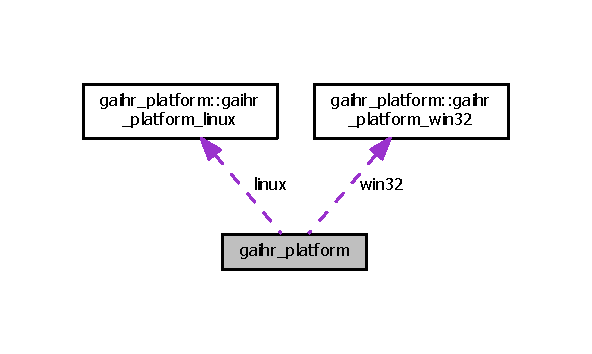
\includegraphics[width=284pt]{uniongaihr__platform__coll__graph}
\end{center}
\end{figure}
\begin{DoxyFields}{Class Members}
\mbox{\Hypertarget{gai__hotreload_8h_aff9109eeb79bcbee6ddf4eab05477a83}\label{gai__hotreload_8h_aff9109eeb79bcbee6ddf4eab05477a83}} 
struct \hyperlink{gai__hotreload_8h_structgaihr__platform_1_1gaihr__platform__linux}{gaihr\_platform\_linux}&
linux&
\\
\hline

\mbox{\Hypertarget{gai__hotreload_8h_ab100a9280dca047d4c625cbf6ea7e64c}\label{gai__hotreload_8h_ab100a9280dca047d4c625cbf6ea7e64c}} 
struct \hyperlink{gai__hotreload_8h_structgaihr__platform_1_1gaihr__platform__win32}{gaihr\_platform\_win32}&
win32&
\\
\hline

\end{DoxyFields}
\index{gaihr\+\_\+platform\+::gaihr\+\_\+platform\+\_\+win32@{gaihr\+\_\+platform\+::gaihr\+\_\+platform\+\_\+win32}}\label{structgaihr__platform_1_1gaihr__platform__win32}
\Hypertarget{gai__hotreload_8h_structgaihr__platform_1_1gaihr__platform__win32}
\subsubsection{struct gaihr\+\_\+platform\+:\+:gaihr\+\_\+platform\+\_\+win32}
\begin{DoxyFields}{Class Members}
\mbox{\Hypertarget{gai__hotreload_8h_aa9b31d30dfd3fa64e40b7cd771f98253}\label{gai__hotreload_8h_aa9b31d30dfd3fa64e40b7cd771f98253}} 
HANDLE&
event&
\\
\hline

\mbox{\Hypertarget{gai__hotreload_8h_ab17cd0ffa18b4ef60cd0d4736f0abc0a}\label{gai__hotreload_8h_ab17cd0ffa18b4ef60cd0d4736f0abc0a}} 
HANDLE&
mutex&
\\
\hline

\end{DoxyFields}
\index{gaihr\+\_\+platform\+::gaihr\+\_\+platform\+\_\+linux@{gaihr\+\_\+platform\+::gaihr\+\_\+platform\+\_\+linux}}\label{structgaihr__platform_1_1gaihr__platform__linux}
\Hypertarget{gai__hotreload_8h_structgaihr__platform_1_1gaihr__platform__linux}
\subsubsection{struct gaihr\+\_\+platform\+:\+:gaihr\+\_\+platform\+\_\+linux}
\begin{DoxyFields}{Class Members}
\mbox{\Hypertarget{gai__hotreload_8h_a50324e3fd2b5fdcfd27f1ae040656ac2}\label{gai__hotreload_8h_a50324e3fd2b5fdcfd27f1ae040656ac2}} 
void $\ast$&
event&
\\
\hline

\mbox{\Hypertarget{gai__hotreload_8h_a02af0c94ad547b2616feff49dcee343e}\label{gai__hotreload_8h_a02af0c94ad547b2616feff49dcee343e}} 
void $\ast$&
mutex&
\\
\hline

\end{DoxyFields}
\index{gaihr\+\_\+file@{gaihr\+\_\+file}}\label{structgaihr__file}
\Hypertarget{gai__hotreload_8h_structgaihr__file}
\subsubsection{struct gaihr\+\_\+file}
\begin{DoxyRefDesc}{Todo}
\item[\hyperlink{todo__todo000001}{Todo}]Think about a way of easily support other platforms. \end{DoxyRefDesc}
\begin{Desc}
\item[Examples\+: ]\par
\hyperlink{hotreload_0Cwin32_0Cmain_8cpp-example}{hotreload\textbackslash{}win32\textbackslash{}main.\+cpp}.\end{Desc}


Collaboration diagram for gaihr\+\_\+file\+:\nopagebreak
\begin{figure}[H]
\begin{center}
\leavevmode
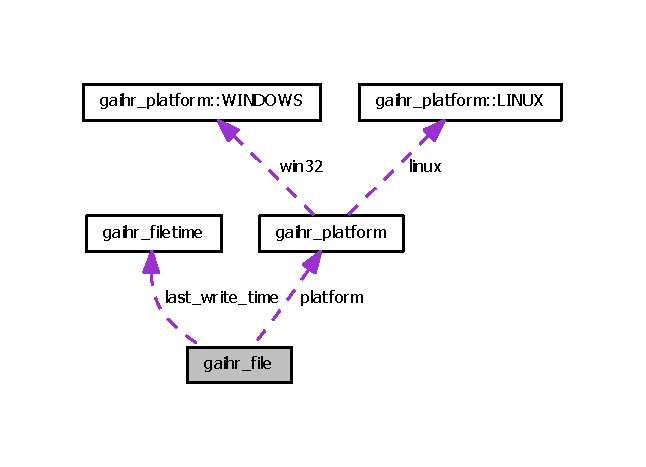
\includegraphics[width=299pt]{structgaihr__file__coll__graph}
\end{center}
\end{figure}
\begin{DoxyFields}{Class Members}
\mbox{\Hypertarget{gai__hotreload_8h_a9ac45c0142ff1eaf591b870e163d7f31}\label{gai__hotreload_8h_a9ac45c0142ff1eaf591b870e163d7f31}} 
\hyperlink{gai__hotreload_8h_a8026f464cf8636b763b6f03798d40800}{gaihr\_callback} $\ast$&
callback&
Callback to the function when an event happens. See \hyperlink{gai__hotreload_8h_a6f8c5bfe220445bbbb8e1c9ef176838a}{G\+A\+I\+H\+R\+\_\+\+C\+A\+L\+L\+B\+A\+CK} \\
\hline

\mbox{\Hypertarget{gai__hotreload_8h_a26ea2bbf62231c3cae2317ca217f8166}\label{gai__hotreload_8h_a26ea2bbf62231c3cae2317ca217f8166}} 
const char $\ast$&
filename&
File to check for changes. \\
\hline

\mbox{\Hypertarget{gai__hotreload_8h_ab6eef82d50a8a51d161de3ab7ad98ee9}\label{gai__hotreload_8h_ab6eef82d50a8a51d161de3ab7ad98ee9}} 
\hyperlink{gai__hotreload_8h_aaebb069b6896f065efd75640e0e4150b}{gaihr\_flags}&
flags&
Flags to specify event handling and callback behaviour. \\
\hline

\mbox{\Hypertarget{gai__hotreload_8h_a38b2bc43116a1fd59715ca1714d80462}\label{gai__hotreload_8h_a38b2bc43116a1fd59715ca1714d80462}} 
\hyperlink{gai__hotreload_8h_uniongaihr__filetime}{gaihr\_filetime}&
last\_write\_time&
Filetime structure. \\
\hline

\mbox{\Hypertarget{gai__hotreload_8h_a138044c270d5f0e83917ae2841efe8b7}\label{gai__hotreload_8h_a138044c270d5f0e83917ae2841efe8b7}} 
\hyperlink{gai__hotreload_8h_uniongaihr__platform}{gaihr\_platform}&
platform&
Platform specfic structure for semaphore or mutex handles. \\
\hline

\mbox{\Hypertarget{gai__hotreload_8h_a06bf963cb9c08e69fcc6c4bb3140a2b8}\label{gai__hotreload_8h_a06bf963cb9c08e69fcc6c4bb3140a2b8}} 
void $\ast$&
userdata&
User passed data. \\
\hline

\end{DoxyFields}
\index{gaihr\+\_\+filetime.\+parts@{gaihr\+\_\+filetime.\+parts}}\label{structgaihr__filetime_8parts}
\Hypertarget{gai__hotreload_8h_structgaihr__filetime_8parts}
\subsubsection{struct gaihr\+\_\+filetime.\+parts}
\begin{DoxyFields}{Class Members}
\mbox{\Hypertarget{gai__hotreload_8h_a8d966b2253a917086c8604959e152243}\label{gai__hotreload_8h_a8d966b2253a917086c8604959e152243}} 
long&
high&
\\
\hline

\mbox{\Hypertarget{gai__hotreload_8h_a53cced8d281a1a0ace3cb6594daaa4f7}\label{gai__hotreload_8h_a53cced8d281a1a0ace3cb6594daaa4f7}} 
long&
low&
\\
\hline

\end{DoxyFields}


\subsection{Macro Definition Documentation}
\mbox{\Hypertarget{gai__hotreload_8h_a11e965cbb3e2af8ed1888b0c6b2777da}\label{gai__hotreload_8h_a11e965cbb3e2af8ed1888b0c6b2777da}} 
\index{gai\+\_\+hotreload.\+h@{gai\+\_\+hotreload.\+h}!G\+A\+I\+H\+R\+\_\+\+A\+S\+S\+E\+RT@{G\+A\+I\+H\+R\+\_\+\+A\+S\+S\+E\+RT}}
\index{G\+A\+I\+H\+R\+\_\+\+A\+S\+S\+E\+RT@{G\+A\+I\+H\+R\+\_\+\+A\+S\+S\+E\+RT}!gai\+\_\+hotreload.\+h@{gai\+\_\+hotreload.\+h}}
\subsubsection{\texorpdfstring{G\+A\+I\+H\+R\+\_\+\+A\+S\+S\+E\+RT}{GAIHR\_ASSERT}}
{\footnotesize\ttfamily \#define G\+A\+I\+H\+R\+\_\+\+A\+S\+S\+E\+RT(\begin{DoxyParamCaption}\item[{}]{cond }\end{DoxyParamCaption})~assert(cond)}



Define {\bfseries G\+A\+I\+H\+R\+\_\+\+A\+S\+S\+E\+RT} before including this file to {\bfseries disable} assertions. 

\begin{DoxyNote}{Note}
Uses assert() from the c-\/standard library by default $<$assert.\+h$>$ 
\end{DoxyNote}

\begin{DoxyParams}{Parameters}
{\em cond} & Assertion condition \\
\hline
\end{DoxyParams}
\mbox{\Hypertarget{gai__hotreload_8h_a6f8c5bfe220445bbbb8e1c9ef176838a}\label{gai__hotreload_8h_a6f8c5bfe220445bbbb8e1c9ef176838a}} 
\index{gai\+\_\+hotreload.\+h@{gai\+\_\+hotreload.\+h}!G\+A\+I\+H\+R\+\_\+\+C\+A\+L\+L\+B\+A\+CK@{G\+A\+I\+H\+R\+\_\+\+C\+A\+L\+L\+B\+A\+CK}}
\index{G\+A\+I\+H\+R\+\_\+\+C\+A\+L\+L\+B\+A\+CK@{G\+A\+I\+H\+R\+\_\+\+C\+A\+L\+L\+B\+A\+CK}!gai\+\_\+hotreload.\+h@{gai\+\_\+hotreload.\+h}}
\subsubsection{\texorpdfstring{G\+A\+I\+H\+R\+\_\+\+C\+A\+L\+L\+B\+A\+CK}{GAIHR\_CALLBACK}}
{\footnotesize\ttfamily \#define G\+A\+I\+H\+R\+\_\+\+C\+A\+L\+L\+B\+A\+CK(\begin{DoxyParamCaption}\item[{}]{name }\end{DoxyParamCaption})~void name(\hyperlink{gai__hotreload_8h_structgaihr__file}{gaihr\+\_\+file} $\ast$file)}



Callback function macro which will generate a function as specified by \hyperlink{gai__hotreload_8h_a8026f464cf8636b763b6f03798d40800}{gaihr\+\_\+callback}. 

{\bfseries Usage} {\bfseries example\+:} 
\begin{DoxyCode}
\hyperlink{gai__hotreload_8h_a6f8c5bfe220445bbbb8e1c9ef176838a}{GAIHR\_CALLBACK}(myCallbackFunction)
\{
        \textcolor{comment}{// Do whatever you want here}
        printf(\textcolor{stringliteral}{"%s\(\backslash\)n"}, file->filename);
\}
\end{DoxyCode}


The above example will actually generate a function which looks like this\+: 
\begin{DoxyCode}
\textcolor{keywordtype}{void} myCallbackFunction(\hyperlink{gai__hotreload_8h_structgaihr__file}{gaihr\_file} *file)
\{
        \textcolor{comment}{// Do whatever you want here}
        printf(\textcolor{stringliteral}{"%s\(\backslash\)n"}, file->\hyperlink{gai__hotreload_8h_a26ea2bbf62231c3cae2317ca217f8166}{filename});
\}
\end{DoxyCode}


See the \hyperlink{gai__hotreload_8h_gaihr_code_example}{Example Code} section for a simple demonstration. \begin{Desc}
\item[Examples\+: ]\par
\hyperlink{hotreload_0Cwin32_0Cmain_8cpp-example}{hotreload\textbackslash{}win32\textbackslash{}main.\+cpp}.\end{Desc}
\mbox{\Hypertarget{gai__hotreload_8h_ac26b515249679c1f9036430164867ba0}\label{gai__hotreload_8h_ac26b515249679c1f9036430164867ba0}} 
\index{gai\+\_\+hotreload.\+h@{gai\+\_\+hotreload.\+h}!G\+A\+I\+H\+R\+\_\+\+F\+I\+L\+E\+\_\+\+L\+I\+M\+IT@{G\+A\+I\+H\+R\+\_\+\+F\+I\+L\+E\+\_\+\+L\+I\+M\+IT}}
\index{G\+A\+I\+H\+R\+\_\+\+F\+I\+L\+E\+\_\+\+L\+I\+M\+IT@{G\+A\+I\+H\+R\+\_\+\+F\+I\+L\+E\+\_\+\+L\+I\+M\+IT}!gai\+\_\+hotreload.\+h@{gai\+\_\+hotreload.\+h}}
\subsubsection{\texorpdfstring{G\+A\+I\+H\+R\+\_\+\+F\+I\+L\+E\+\_\+\+L\+I\+M\+IT}{GAIHR\_FILE\_LIMIT}}
{\footnotesize\ttfamily \#define G\+A\+I\+H\+R\+\_\+\+F\+I\+L\+E\+\_\+\+L\+I\+M\+IT~64}

Max files which will be processed by the worker thread. Note\+: Will be replaced by a linked list! \mbox{\Hypertarget{gai__hotreload_8h_a7385b7149ef022fa38140e2b2a540502}\label{gai__hotreload_8h_a7385b7149ef022fa38140e2b2a540502}} 
\index{gai\+\_\+hotreload.\+h@{gai\+\_\+hotreload.\+h}!G\+A\+I\+H\+R\+\_\+\+T\+H\+R\+E\+A\+D\+\_\+\+T\+I\+M\+E\+O\+UT@{G\+A\+I\+H\+R\+\_\+\+T\+H\+R\+E\+A\+D\+\_\+\+T\+I\+M\+E\+O\+UT}}
\index{G\+A\+I\+H\+R\+\_\+\+T\+H\+R\+E\+A\+D\+\_\+\+T\+I\+M\+E\+O\+UT@{G\+A\+I\+H\+R\+\_\+\+T\+H\+R\+E\+A\+D\+\_\+\+T\+I\+M\+E\+O\+UT}!gai\+\_\+hotreload.\+h@{gai\+\_\+hotreload.\+h}}
\subsubsection{\texorpdfstring{G\+A\+I\+H\+R\+\_\+\+T\+H\+R\+E\+A\+D\+\_\+\+T\+I\+M\+E\+O\+UT}{GAIHR\_THREAD\_TIMEOUT}}
{\footnotesize\ttfamily \#define G\+A\+I\+H\+R\+\_\+\+T\+H\+R\+E\+A\+D\+\_\+\+T\+I\+M\+E\+O\+UT~1000}

Thread sleeping time until it checks for updated files again \mbox{\Hypertarget{gai__hotreload_8h_a36b03891b740d035afdd1f32e15c91ad}\label{gai__hotreload_8h_a36b03891b740d035afdd1f32e15c91ad}} 
\index{gai\+\_\+hotreload.\+h@{gai\+\_\+hotreload.\+h}!G\+A\+I\+H\+R\+\_\+\+W\+A\+I\+T\+\_\+\+I\+N\+F\+I\+N\+I\+TE@{G\+A\+I\+H\+R\+\_\+\+W\+A\+I\+T\+\_\+\+I\+N\+F\+I\+N\+I\+TE}}
\index{G\+A\+I\+H\+R\+\_\+\+W\+A\+I\+T\+\_\+\+I\+N\+F\+I\+N\+I\+TE@{G\+A\+I\+H\+R\+\_\+\+W\+A\+I\+T\+\_\+\+I\+N\+F\+I\+N\+I\+TE}!gai\+\_\+hotreload.\+h@{gai\+\_\+hotreload.\+h}}
\subsubsection{\texorpdfstring{G\+A\+I\+H\+R\+\_\+\+W\+A\+I\+T\+\_\+\+I\+N\+F\+I\+N\+I\+TE}{GAIHR\_WAIT\_INFINITE}}
{\footnotesize\ttfamily \#define G\+A\+I\+H\+R\+\_\+\+W\+A\+I\+T\+\_\+\+I\+N\+F\+I\+N\+I\+TE~-\/1}

Note\+: Currently the windows specified value for I\+N\+F\+I\+N\+I\+TE. Will possibly be changed! 

\subsection{Enumeration Type Documentation}
\mbox{\Hypertarget{gai__hotreload_8h_aaebb069b6896f065efd75640e0e4150b}\label{gai__hotreload_8h_aaebb069b6896f065efd75640e0e4150b}} 
\index{gai\+\_\+hotreload.\+h@{gai\+\_\+hotreload.\+h}!gaihr\+\_\+flags@{gaihr\+\_\+flags}}
\index{gaihr\+\_\+flags@{gaihr\+\_\+flags}!gai\+\_\+hotreload.\+h@{gai\+\_\+hotreload.\+h}}
\subsubsection{\texorpdfstring{gaihr\+\_\+flags}{gaihr\_flags}}
{\footnotesize\ttfamily enum \hyperlink{gai__hotreload_8h_aaebb069b6896f065efd75640e0e4150b}{gaihr\+\_\+flags}}



This flags specify how the event and callback function will be handled. 

\begin{DoxyEnumFields}{Enumerator}
\raisebox{\heightof{T}}[0pt][0pt]{\index{gaihr\+\_\+\+Flags\+None@{gaihr\+\_\+\+Flags\+None}!gai\+\_\+hotreload.\+h@{gai\+\_\+hotreload.\+h}}\index{gai\+\_\+hotreload.\+h@{gai\+\_\+hotreload.\+h}!gaihr\+\_\+\+Flags\+None@{gaihr\+\_\+\+Flags\+None}}}\mbox{\Hypertarget{gai__hotreload_8h_aaebb069b6896f065efd75640e0e4150ba6c207a28fdce6637b4aa1e70e64c3e94}\label{gai__hotreload_8h_aaebb069b6896f065efd75640e0e4150ba6c207a28fdce6637b4aa1e70e64c3e94}} 
gaihr\+\_\+\+Flags\+None&Nothing specified. \\
\hline

\raisebox{\heightof{T}}[0pt][0pt]{\index{gaihr\+\_\+\+Flags\+Dont\+Handle\+Event@{gaihr\+\_\+\+Flags\+Dont\+Handle\+Event}!gai\+\_\+hotreload.\+h@{gai\+\_\+hotreload.\+h}}\index{gai\+\_\+hotreload.\+h@{gai\+\_\+hotreload.\+h}!gaihr\+\_\+\+Flags\+Dont\+Handle\+Event@{gaihr\+\_\+\+Flags\+Dont\+Handle\+Event}}}\mbox{\Hypertarget{gai__hotreload_8h_aaebb069b6896f065efd75640e0e4150ba158375938f45efe930ee7416d19e5a6c}\label{gai__hotreload_8h_aaebb069b6896f065efd75640e0e4150ba158375938f45efe930ee7416d19e5a6c}} 
gaihr\+\_\+\+Flags\+Dont\+Handle\+Event&Indicates whether the thread will not call the callback function on event. You should call it yourself! \\
\hline

\raisebox{\heightof{T}}[0pt][0pt]{\index{gaihr\+\_\+\+Flags\+Dont\+Reset\+Event@{gaihr\+\_\+\+Flags\+Dont\+Reset\+Event}!gai\+\_\+hotreload.\+h@{gai\+\_\+hotreload.\+h}}\index{gai\+\_\+hotreload.\+h@{gai\+\_\+hotreload.\+h}!gaihr\+\_\+\+Flags\+Dont\+Reset\+Event@{gaihr\+\_\+\+Flags\+Dont\+Reset\+Event}}}\mbox{\Hypertarget{gai__hotreload_8h_aaebb069b6896f065efd75640e0e4150babfc4c1c7557333f4e2cddf40cacefc7a}\label{gai__hotreload_8h_aaebb069b6896f065efd75640e0e4150babfc4c1c7557333f4e2cddf40cacefc7a}} 
gaihr\+\_\+\+Flags\+Dont\+Reset\+Event&Indicates whether the marked event will not be resetted after calling the callback function. You have to do reset it yourself! \\
\hline

\raisebox{\heightof{T}}[0pt][0pt]{\index{gaihr\+\_\+\+Flags\+Skip\+Initial\+Change@{gaihr\+\_\+\+Flags\+Skip\+Initial\+Change}!gai\+\_\+hotreload.\+h@{gai\+\_\+hotreload.\+h}}\index{gai\+\_\+hotreload.\+h@{gai\+\_\+hotreload.\+h}!gaihr\+\_\+\+Flags\+Skip\+Initial\+Change@{gaihr\+\_\+\+Flags\+Skip\+Initial\+Change}}}\mbox{\Hypertarget{gai__hotreload_8h_aaebb069b6896f065efd75640e0e4150baee50ce1492a508e5605592106fa00bd5}\label{gai__hotreload_8h_aaebb069b6896f065efd75640e0e4150baee50ce1492a508e5605592106fa00bd5}} 
gaihr\+\_\+\+Flags\+Skip\+Initial\+Change&Indicates whether the initial file change will not result in an event. \\
\hline

\end{DoxyEnumFields}


\subsection{Function Documentation}
\mbox{\Hypertarget{gai__hotreload_8h_a52aa011dc92eb63b9d5fc7993042eb3f}\label{gai__hotreload_8h_a52aa011dc92eb63b9d5fc7993042eb3f}} 
\index{gai\+\_\+hotreload.\+h@{gai\+\_\+hotreload.\+h}!\+\_\+gaihr\+\_\+\+Begin\+Ticket\+Mutex@{\+\_\+gaihr\+\_\+\+Begin\+Ticket\+Mutex}}
\index{\+\_\+gaihr\+\_\+\+Begin\+Ticket\+Mutex@{\+\_\+gaihr\+\_\+\+Begin\+Ticket\+Mutex}!gai\+\_\+hotreload.\+h@{gai\+\_\+hotreload.\+h}}
\subsubsection{\texorpdfstring{\+\_\+gaihr\+\_\+\+Begin\+Ticket\+Mutex()}{\_gaihr\_BeginTicketMutex()}}
{\footnotesize\ttfamily \hyperlink{gai__hotreload_8h_a32983003a4e816a8350f01cb22d1b01b}{G\+A\+I\+H\+R\+\_\+\+A\+PI} unsigned int \+\_\+gaihr\+\_\+\+Begin\+Ticket\+Mutex (\begin{DoxyParamCaption}\item[{\hyperlink{gai__hotreload_8h_structgaihr__file}{gaihr\+\_\+file} $\ast$}]{file,  }\item[{int}]{timeout = {\ttfamily \hyperlink{gai__hotreload_8h_a36b03891b740d035afdd1f32e15c91ad}{G\+A\+I\+H\+R\+\_\+\+W\+A\+I\+T\+\_\+\+I\+N\+F\+I\+N\+I\+TE}} }\end{DoxyParamCaption})}



Opens a mutex to access the data safely in a multi-\/threaded way. 


\begin{DoxyParams}{Parameters}
{\em file} & Handle to a \hyperlink{gai__hotreload_8h_structgaihr__file}{gaihr\+\_\+file} instance. \\
\hline
{\em timeout} & Time to grab the mutex. (Can take longer if the mutex is used by another thread and was not released yet!) \\
\hline
\end{DoxyParams}
\begin{DoxyReturn}{Returns}
\tabulinesep=1mm
\begin{longtabu} spread 0pt [c]{*{2}{|X[-1]}|}
\hline
\rowcolor{\tableheadbgcolor}\textbf{ Return Code }&\textbf{ Description  }\\\cline{1-2}
\endfirsthead
\hline
\endfoot
\hline
\rowcolor{\tableheadbgcolor}\textbf{ Return Code }&\textbf{ Description  }\\\cline{1-2}
\endhead
1 &Mutex was succesfully opened \\\cline{1-2}
0 &Failure (mutex is probably used by another thread) \\\cline{1-2}
\end{longtabu}

\end{DoxyReturn}
\mbox{\Hypertarget{gai__hotreload_8h_acee43647e5f69a31c40726d43bfe19e3}\label{gai__hotreload_8h_acee43647e5f69a31c40726d43bfe19e3}} 
\index{gai\+\_\+hotreload.\+h@{gai\+\_\+hotreload.\+h}!\+\_\+gaihr\+\_\+\+Compare\+File\+Time@{\+\_\+gaihr\+\_\+\+Compare\+File\+Time}}
\index{\+\_\+gaihr\+\_\+\+Compare\+File\+Time@{\+\_\+gaihr\+\_\+\+Compare\+File\+Time}!gai\+\_\+hotreload.\+h@{gai\+\_\+hotreload.\+h}}
\subsubsection{\texorpdfstring{\+\_\+gaihr\+\_\+\+Compare\+File\+Time()}{\_gaihr\_CompareFileTime()}}
{\footnotesize\ttfamily \hyperlink{gai__hotreload_8h_a32983003a4e816a8350f01cb22d1b01b}{G\+A\+I\+H\+R\+\_\+\+A\+PI} int \+\_\+gaihr\+\_\+\+Compare\+File\+Time (\begin{DoxyParamCaption}\item[{\hyperlink{gai__hotreload_8h_uniongaihr__filetime}{gaihr\+\_\+filetime} $\ast$}]{a,  }\item[{\hyperlink{gai__hotreload_8h_uniongaihr__filetime}{gaihr\+\_\+filetime} $\ast$}]{b }\end{DoxyParamCaption})}



Compare two gaihr\+\_\+filetimes to each other. 


\begin{DoxyParams}{Parameters}
{\em a} & A pointer to a \hyperlink{gai__hotreload_8h_uniongaihr__filetime}{gaihr\+\_\+filetime} structure \\
\hline
{\em b} & A pointer to a \hyperlink{gai__hotreload_8h_uniongaihr__filetime}{gaihr\+\_\+filetime} structure\\
\hline
\end{DoxyParams}
\begin{DoxyReturn}{Returns}
\tabulinesep=1mm
\begin{longtabu} spread 0pt [c]{*{2}{|X[-1]}|}
\hline
\rowcolor{\tableheadbgcolor}\textbf{ Return Code }&\textbf{ Description  }\\\cline{1-2}
\endfirsthead
\hline
\endfoot
\hline
\rowcolor{\tableheadbgcolor}\textbf{ Return Code }&\textbf{ Description  }\\\cline{1-2}
\endhead
-\/1 &a is higher than b \\\cline{1-2}
0 &a equals b \\\cline{1-2}
1 &b is higher than a \\\cline{1-2}
\end{longtabu}

\end{DoxyReturn}
\mbox{\Hypertarget{gai__hotreload_8h_a7017705231a1470b0a03c14a9c28aa11}\label{gai__hotreload_8h_a7017705231a1470b0a03c14a9c28aa11}} 
\index{gai\+\_\+hotreload.\+h@{gai\+\_\+hotreload.\+h}!\+\_\+gaihr\+\_\+\+Do\+Work@{\+\_\+gaihr\+\_\+\+Do\+Work}}
\index{\+\_\+gaihr\+\_\+\+Do\+Work@{\+\_\+gaihr\+\_\+\+Do\+Work}!gai\+\_\+hotreload.\+h@{gai\+\_\+hotreload.\+h}}
\subsubsection{\texorpdfstring{\+\_\+gaihr\+\_\+\+Do\+Work()}{\_gaihr\_DoWork()}}
{\footnotesize\ttfamily \hyperlink{gai__hotreload_8h_a32983003a4e816a8350f01cb22d1b01b}{G\+A\+I\+H\+R\+\_\+\+A\+PI} void \+\_\+gaihr\+\_\+\+Do\+Work (\begin{DoxyParamCaption}\item[{\hyperlink{gai__hotreload_8h_structgaihr__file}{gaihr\+\_\+file} $\ast$$\ast$}]{files }\end{DoxyParamCaption})}



Loops through all files to track. 


\begin{DoxyParams}{Parameters}
{\em files} & A pointer to an array of \hyperlink{gai__hotreload_8h_structgaihr__file}{gaihr\+\_\+file} structures \\
\hline
\end{DoxyParams}
\mbox{\Hypertarget{gai__hotreload_8h_ae6e501372d35a3645332dadb8f612e3c}\label{gai__hotreload_8h_ae6e501372d35a3645332dadb8f612e3c}} 
\index{gai\+\_\+hotreload.\+h@{gai\+\_\+hotreload.\+h}!\+\_\+gaihr\+\_\+\+End\+Ticket\+Mutex@{\+\_\+gaihr\+\_\+\+End\+Ticket\+Mutex}}
\index{\+\_\+gaihr\+\_\+\+End\+Ticket\+Mutex@{\+\_\+gaihr\+\_\+\+End\+Ticket\+Mutex}!gai\+\_\+hotreload.\+h@{gai\+\_\+hotreload.\+h}}
\subsubsection{\texorpdfstring{\+\_\+gaihr\+\_\+\+End\+Ticket\+Mutex()}{\_gaihr\_EndTicketMutex()}}
{\footnotesize\ttfamily \hyperlink{gai__hotreload_8h_a32983003a4e816a8350f01cb22d1b01b}{G\+A\+I\+H\+R\+\_\+\+A\+PI} void \+\_\+gaihr\+\_\+\+End\+Ticket\+Mutex (\begin{DoxyParamCaption}\item[{\hyperlink{gai__hotreload_8h_structgaihr__file}{gaihr\+\_\+file} $\ast$}]{file }\end{DoxyParamCaption})}



Releases the previously opened mutex to allow other thread to use this mutex. 


\begin{DoxyParams}{Parameters}
{\em file} & Handle to a \hyperlink{gai__hotreload_8h_structgaihr__file}{gaihr\+\_\+file} instance. \\
\hline
\end{DoxyParams}
\mbox{\Hypertarget{gai__hotreload_8h_aba347f4afef1dd5f850142adf487fa26}\label{gai__hotreload_8h_aba347f4afef1dd5f850142adf487fa26}} 
\index{gai\+\_\+hotreload.\+h@{gai\+\_\+hotreload.\+h}!\+\_\+gaihr\+\_\+\+Reset\+Event@{\+\_\+gaihr\+\_\+\+Reset\+Event}}
\index{\+\_\+gaihr\+\_\+\+Reset\+Event@{\+\_\+gaihr\+\_\+\+Reset\+Event}!gai\+\_\+hotreload.\+h@{gai\+\_\+hotreload.\+h}}
\subsubsection{\texorpdfstring{\+\_\+gaihr\+\_\+\+Reset\+Event()}{\_gaihr\_ResetEvent()}}
{\footnotesize\ttfamily \hyperlink{gai__hotreload_8h_a32983003a4e816a8350f01cb22d1b01b}{G\+A\+I\+H\+R\+\_\+\+A\+PI} void \+\_\+gaihr\+\_\+\+Reset\+Event (\begin{DoxyParamCaption}\item[{\hyperlink{gai__hotreload_8h_structgaihr__file}{gaihr\+\_\+file} $\ast$}]{file }\end{DoxyParamCaption})}



Resets the previously set signal. 


\begin{DoxyParams}{Parameters}
{\em file} & Handle to a \hyperlink{gai__hotreload_8h_structgaihr__file}{gaihr\+\_\+file} instance. \\
\hline
\end{DoxyParams}
\mbox{\Hypertarget{gai__hotreload_8h_a465162f1865f5f804311c153c0995543}\label{gai__hotreload_8h_a465162f1865f5f804311c153c0995543}} 
\index{gai\+\_\+hotreload.\+h@{gai\+\_\+hotreload.\+h}!\+\_\+gaihr\+\_\+\+Set\+Event@{\+\_\+gaihr\+\_\+\+Set\+Event}}
\index{\+\_\+gaihr\+\_\+\+Set\+Event@{\+\_\+gaihr\+\_\+\+Set\+Event}!gai\+\_\+hotreload.\+h@{gai\+\_\+hotreload.\+h}}
\subsubsection{\texorpdfstring{\+\_\+gaihr\+\_\+\+Set\+Event()}{\_gaihr\_SetEvent()}}
{\footnotesize\ttfamily \hyperlink{gai__hotreload_8h_a32983003a4e816a8350f01cb22d1b01b}{G\+A\+I\+H\+R\+\_\+\+A\+PI} void \+\_\+gaihr\+\_\+\+Set\+Event (\begin{DoxyParamCaption}\item[{\hyperlink{gai__hotreload_8h_structgaihr__file}{gaihr\+\_\+file} $\ast$}]{file }\end{DoxyParamCaption})}



Signals a file change to the user. 


\begin{DoxyParams}{Parameters}
{\em file} & Handle to a \hyperlink{gai__hotreload_8h_structgaihr__file}{gaihr\+\_\+file} instance. \\
\hline
\end{DoxyParams}
\mbox{\Hypertarget{gai__hotreload_8h_ad83d8f6170f0404fb72803d012ac9f6a}\label{gai__hotreload_8h_ad83d8f6170f0404fb72803d012ac9f6a}} 
\index{gai\+\_\+hotreload.\+h@{gai\+\_\+hotreload.\+h}!gaihr\+\_\+\+Track@{gaihr\+\_\+\+Track}}
\index{gaihr\+\_\+\+Track@{gaihr\+\_\+\+Track}!gai\+\_\+hotreload.\+h@{gai\+\_\+hotreload.\+h}}
\subsubsection{\texorpdfstring{gaihr\+\_\+\+Track()}{gaihr\_Track()}}
{\footnotesize\ttfamily \hyperlink{gai__hotreload_8h_a32983003a4e816a8350f01cb22d1b01b}{G\+A\+I\+H\+R\+\_\+\+A\+PI} unsigned int gaihr\+\_\+\+Track (\begin{DoxyParamCaption}\item[{\hyperlink{gai__hotreload_8h_structgaihr__file}{gaihr\+\_\+file} $\ast$}]{file,  }\item[{const char $\ast$}]{filename,  }\item[{\hyperlink{gai__hotreload_8h_a8026f464cf8636b763b6f03798d40800}{gaihr\+\_\+callback} $\ast$}]{callback = {\ttfamily 0},  }\item[{void $\ast$}]{userdata = {\ttfamily 0},  }\item[{\hyperlink{gai__hotreload_8h_aaebb069b6896f065efd75640e0e4150b}{gaihr\+\_\+flags}}]{flags = {\ttfamily \hyperlink{gai__hotreload_8h_aaebb069b6896f065efd75640e0e4150ba6c207a28fdce6637b4aa1e70e64c3e94}{gaihr\+\_\+\+Flags\+None}} }\end{DoxyParamCaption})}



Adds a file to a worker thread, which internally tracks if the given file was modified. If so it will fire an event which will result in a function call to the callback function or handled differently depending on the specified flags. 


\begin{DoxyParams}{Parameters}
{\em file} & A pointer to a \hyperlink{gai__hotreload_8h_structgaihr__file}{gaihr\+\_\+file} structure. \\
\hline
{\em filename} & Filename of the file to track (relative or full). \\
\hline
{\em callback} & (optional) A pointer to he callback function. See \hyperlink{gai__hotreload_8h_a6f8c5bfe220445bbbb8e1c9ef176838a}{G\+A\+I\+H\+R\+\_\+\+C\+A\+L\+L\+B\+A\+CK} \\
\hline
{\em userdata} & (optional) A pointer to userdefined memory. \\
\hline
{\em flags} & (optional) Flags to handle events and callbacks. See \hyperlink{gai__hotreload_8h_aaebb069b6896f065efd75640e0e4150b}{gaihr\+\_\+flags} \\
\hline
\end{DoxyParams}
\begin{DoxyReturn}{Returns}
\tabulinesep=1mm
\begin{longtabu} spread 0pt [c]{*{2}{|X[-1]}|}
\hline
\rowcolor{\tableheadbgcolor}\textbf{ Return Code }&\textbf{ Description  }\\\cline{1-2}
\endfirsthead
\hline
\endfoot
\hline
\rowcolor{\tableheadbgcolor}\textbf{ Return Code }&\textbf{ Description  }\\\cline{1-2}
\endhead
1 &Success \\\cline{1-2}
0 &Failure \\\cline{1-2}
\end{longtabu}

\end{DoxyReturn}
\begin{Desc}
\item[Examples\+: ]\par
\hyperlink{hotreload_0Cwin32_0Cmain_8cpp-example}{hotreload\textbackslash{}win32\textbackslash{}main.\+cpp}.\end{Desc}
\mbox{\Hypertarget{gai__hotreload_8h_a288369c901929574624b267de90007cd}\label{gai__hotreload_8h_a288369c901929574624b267de90007cd}} 
\index{gai\+\_\+hotreload.\+h@{gai\+\_\+hotreload.\+h}!gaihr\+\_\+\+Untrack@{gaihr\+\_\+\+Untrack}}
\index{gaihr\+\_\+\+Untrack@{gaihr\+\_\+\+Untrack}!gai\+\_\+hotreload.\+h@{gai\+\_\+hotreload.\+h}}
\subsubsection{\texorpdfstring{gaihr\+\_\+\+Untrack()}{gaihr\_Untrack()}}
{\footnotesize\ttfamily \hyperlink{gai__hotreload_8h_a32983003a4e816a8350f01cb22d1b01b}{G\+A\+I\+H\+R\+\_\+\+A\+PI} unsigned int gaihr\+\_\+\+Untrack (\begin{DoxyParamCaption}\item[{\hyperlink{gai__hotreload_8h_structgaihr__file}{gaihr\+\_\+file} $\ast$}]{file }\end{DoxyParamCaption})}



Removes a file from the worker thread. 


\begin{DoxyParams}{Parameters}
{\em file} & Handle to a \hyperlink{gai__hotreload_8h_structgaihr__file}{gaihr\+\_\+file} instance. \\
\hline
\end{DoxyParams}
\begin{DoxyReturn}{Returns}
\tabulinesep=1mm
\begin{longtabu} spread 0pt [c]{*{2}{|X[-1]}|}
\hline
\rowcolor{\tableheadbgcolor}\textbf{ Return Code }&\textbf{ Description  }\\\cline{1-2}
\endfirsthead
\hline
\endfoot
\hline
\rowcolor{\tableheadbgcolor}\textbf{ Return Code }&\textbf{ Description  }\\\cline{1-2}
\endhead
1 &Success \\\cline{1-2}
0 &Failure \\\cline{1-2}
\end{longtabu}

\end{DoxyReturn}
\mbox{\Hypertarget{gai__hotreload_8h_a79d4ca28cdaae457474d55a0a21dd326}\label{gai__hotreload_8h_a79d4ca28cdaae457474d55a0a21dd326}} 
\index{gai\+\_\+hotreload.\+h@{gai\+\_\+hotreload.\+h}!gaihr\+\_\+\+Wait\+For\+Event@{gaihr\+\_\+\+Wait\+For\+Event}}
\index{gaihr\+\_\+\+Wait\+For\+Event@{gaihr\+\_\+\+Wait\+For\+Event}!gai\+\_\+hotreload.\+h@{gai\+\_\+hotreload.\+h}}
\subsubsection{\texorpdfstring{gaihr\+\_\+\+Wait\+For\+Event()}{gaihr\_WaitForEvent()}}
{\footnotesize\ttfamily \hyperlink{gai__hotreload_8h_a32983003a4e816a8350f01cb22d1b01b}{G\+A\+I\+H\+R\+\_\+\+A\+PI} void gaihr\+\_\+\+Wait\+For\+Event (\begin{DoxyParamCaption}\item[{\hyperlink{gai__hotreload_8h_structgaihr__file}{gaihr\+\_\+file} $\ast$}]{file }\end{DoxyParamCaption})}



Grabs a mutex for the specified \hyperlink{gai__hotreload_8h_structgaihr__file}{gaihr\+\_\+file} handle and waits for an event. If a callback function is specifed and an event happend the callback function will be called. 


\begin{DoxyParams}{Parameters}
{\em file} & Handle to a \hyperlink{gai__hotreload_8h_structgaihr__file}{gaihr\+\_\+file} instance. \\
\hline
\end{DoxyParams}

\hypertarget{gai__xwindow_8h}{}\section{gai\+\_\+xwindow.\+h File Reference}
\label{gai__xwindow_8h}\index{gai\+\_\+xwindow.\+h@{gai\+\_\+xwindow.\+h}}


Requests a window for all currently supported platforms.  


{\ttfamily \#include $<$assert.\+h$>$}\newline
{\ttfamily \#include $<$string.\+h$>$}\newline
{\ttfamily \#include $<$windows.\+h$>$}\newline
{\ttfamily \#include $<$X11/\+Xlib.\+h$>$}\newline
Include dependency graph for gai\+\_\+xwindow.\+h\+:\nopagebreak
\begin{figure}[H]
\begin{center}
\leavevmode
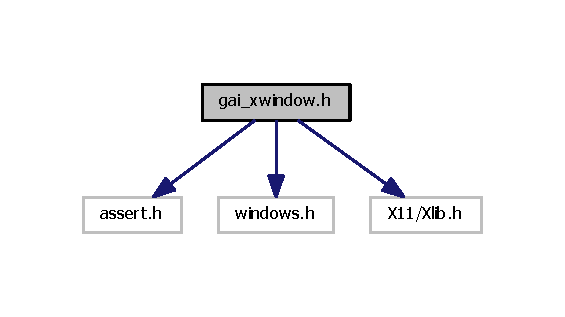
\includegraphics[width=334pt]{gai__xwindow_8h__incl}
\end{center}
\end{figure}
\subsection*{Classes}
\begin{DoxyCompactItemize}
\item 
struct \hyperlink{gai__xwindow_8h_structgaixw__frametime}{gaixw\+\_\+frametime}
\item 
struct \hyperlink{gai__xwindow_8h_structgaixw__info}{gaixw\+\_\+info}
\item 
struct \hyperlink{gai__xwindow_8h_structgaixw__input}{gaixw\+\_\+input}
\item 
struct \hyperlink{gai__xwindow_8h_structgaixw__opengl}{gaixw\+\_\+opengl}
\item 
struct \hyperlink{gai__xwindow_8h_structgaixw__directx}{gaixw\+\_\+directx}
\item 
union \hyperlink{gai__xwindow_8h_uniongaixw__interface}{gaixw\+\_\+interface}
\item 
struct \hyperlink{gai__xwindow_8h_structgaixw__platform__win32}{gaixw\+\_\+platform\+\_\+win32}
\item 
struct \hyperlink{gai__xwindow_8h_structgaixw__platform__linux}{gaixw\+\_\+platform\+\_\+linux}
\item 
union \hyperlink{gai__xwindow_8h_uniongaixw__platform}{gaixw\+\_\+platform}
\item 
struct \hyperlink{gai__xwindow_8h_structgaixw__renderer}{gaixw\+\_\+renderer}
\item 
struct \hyperlink{gai__xwindow_8h_structgaixw__context}{gaixw\+\_\+context}
\end{DoxyCompactItemize}
\subsection*{Macros}
\begin{DoxyCompactItemize}
\item 
\mbox{\Hypertarget{gai__xwindow_8h_ab41ae714bb16012af56329f9032e6d16}\label{gai__xwindow_8h_ab41ae714bb16012af56329f9032e6d16}} 
\#define \hyperlink{gai__xwindow_8h_ab41ae714bb16012af56329f9032e6d16}{G\+A\+I\+X\+W\+\_\+\+A\+PI}~extern
\begin{DoxyCompactList}\small\item\em Define {\bfseries G\+A\+I\+X\+W\+\_\+\+S\+T\+A\+T\+IC} if you want to make functions {\bfseries static} instead of {\bfseries extern} \end{DoxyCompactList}\item 
\#define \hyperlink{gai__xwindow_8h_ab2663b30ef0369cf059d79977b93807f}{G\+A\+I\+X\+W\+\_\+\+A\+S\+S\+E\+RT}(cond)~assert(cond)
\begin{DoxyCompactList}\small\item\em Define {\bfseries G\+A\+I\+X\+W\+\_\+\+A\+S\+S\+E\+RT} before including this file to {\bfseries disable} assertions. \end{DoxyCompactList}\item 
\#define \hyperlink{gai__xwindow_8h_ad52cbaf070ae26059c515d4613a401f4}{G\+A\+I\+X\+W\+\_\+\+P\+R\+I\+NT}(fmt, ...)
\begin{DoxyCompactList}\small\item\em Define this macro before including this file if you want to redirect the output. \end{DoxyCompactList}\item 
\#define \hyperlink{gai__xwindow_8h_aaa1d25d5e0f693faca8ccb08cc744fb6}{G\+A\+I\+X\+W\+\_\+\+C\+L\+A\+S\+S\+N\+A\+ME}~\char`\"{}libgai\+\_\+xwindow\+\_\+framework\char`\"{}
\end{DoxyCompactItemize}
\subsection*{Enumerations}
\begin{DoxyCompactItemize}
\item 
enum \hyperlink{gai__xwindow_8h_a4eae6e51f0425197a4c1010fcc7c8c9d}{gaixw\+\_\+renderer\+\_\+enum} \{ \newline
\hyperlink{gai__xwindow_8h_a4eae6e51f0425197a4c1010fcc7c8c9da25a9a692888d86fd6bf5f24e0c31a8e8}{gaixw\+Renderer\+Unknown}, 
\hyperlink{gai__xwindow_8h_a4eae6e51f0425197a4c1010fcc7c8c9da2ecf0eac74bd3c8d842991bd7c0e15a0}{gaixw\+Renderer\+X11}, 
\hyperlink{gai__xwindow_8h_a4eae6e51f0425197a4c1010fcc7c8c9dab382f06ccd349a4749bfcea4fd5f3080}{gaixw\+Renderer\+G\+DI}, 
\hyperlink{gai__xwindow_8h_a4eae6e51f0425197a4c1010fcc7c8c9da1217be504c773ce47ba76be4ddf9489d}{gaixw\+Renderer\+D\+X10}, 
\newline
\hyperlink{gai__xwindow_8h_a4eae6e51f0425197a4c1010fcc7c8c9dab19a6d88f34235d7333fbc209d1f178a}{gaixw\+Renderer\+D\+X11}, 
\hyperlink{gai__xwindow_8h_a4eae6e51f0425197a4c1010fcc7c8c9da8cd168a752459bca73bdea7b77eb421e}{gaixw\+Renderer\+D\+X12}, 
\hyperlink{gai__xwindow_8h_a4eae6e51f0425197a4c1010fcc7c8c9daf43570fcfedb502e88eb5c69f0eeecc1}{gaixw\+Renderer\+Open\+GL}, 
\hyperlink{gai__xwindow_8h_a4eae6e51f0425197a4c1010fcc7c8c9da4cd9efc9b0b4bcc5674423557a0214ab}{gaixw\+Renderer\+Vulcan}, 
\newline
{\bfseries gaixw\+Renderer\+Max}
 \}\begin{DoxyCompactList}\small\item\em Renderer backend types. \end{DoxyCompactList}
\item 
enum \hyperlink{gai__xwindow_8h_a52d65318fd4fb0d358385d67f156d00c}{gaixw\+\_\+renderer\+\_\+flags} \{ \newline
{\bfseries gaixw\+Flags\+None} = 0x00, 
\hyperlink{gai__xwindow_8h_a52d65318fd4fb0d358385d67f156d00ca024bb28b1d09e6dabb43cca1db088cd1}{gaixw\+Flags\+Minimized} = 0x01, 
\hyperlink{gai__xwindow_8h_a52d65318fd4fb0d358385d67f156d00ca4c1b948394dbf097f6007e01ded11242}{gaixw\+Flags\+Maximized} = 0x02, 
\hyperlink{gai__xwindow_8h_a52d65318fd4fb0d358385d67f156d00ca1b5d286481622b104b8dd24bf3114cd2}{gaixw\+Flags\+Fullscreen} = 0x10, 
\newline
\hyperlink{gai__xwindow_8h_a52d65318fd4fb0d358385d67f156d00ca39f9d8a5253caf225480a80d1b52e4c2}{gaixw\+Flags\+V\+S\+Y\+NC} = 0x20
 \}\begin{DoxyCompactList}\small\item\em Renderer flags. \end{DoxyCompactList}
\end{DoxyCompactItemize}
\subsection*{Functions}
\begin{DoxyCompactItemize}
\item 
\hyperlink{gai__xwindow_8h_ab41ae714bb16012af56329f9032e6d16}{G\+A\+I\+X\+W\+\_\+\+A\+PI} int \hyperlink{gai__xwindow_8h_adec8bb998b6861c4d239b25634c8eb55}{gaixw\+\_\+\+Init} (\hyperlink{gai__xwindow_8h_structgaixw__context}{gaixw\+\_\+context} $\ast$window, const char $\ast$title=\char`\"{}default window title\char`\"{}, int width=-\/1, int height=-\/1, int x=-\/1, int y=-\/1, const char $\ast$classname=\hyperlink{gai__xwindow_8h_aaa1d25d5e0f693faca8ccb08cc744fb6}{G\+A\+I\+X\+W\+\_\+\+C\+L\+A\+S\+S\+N\+A\+ME}, unsigned int visible=1)
\begin{DoxyCompactList}\small\item\em Initializes a window for the current platform. \end{DoxyCompactList}\item 
\hyperlink{gai__xwindow_8h_ab41ae714bb16012af56329f9032e6d16}{G\+A\+I\+X\+W\+\_\+\+A\+PI} void \hyperlink{gai__xwindow_8h_a986353262ac6038b69005bec8111ac56}{gaixw\+\_\+\+Deinit} (\hyperlink{gai__xwindow_8h_structgaixw__context}{gaixw\+\_\+context} $\ast$window)
\begin{DoxyCompactList}\small\item\em Deinitializes the window. \end{DoxyCompactList}\item 
\hyperlink{gai__xwindow_8h_ab41ae714bb16012af56329f9032e6d16}{G\+A\+I\+X\+W\+\_\+\+A\+PI} int \hyperlink{gai__xwindow_8h_aee43c7fda31af1c6808f212e406cebb6}{gaixw\+\_\+\+Show} (\hyperlink{gai__xwindow_8h_structgaixw__context}{gaixw\+\_\+context} $\ast$window)
\begin{DoxyCompactList}\small\item\em Makes the window visible to the user. \end{DoxyCompactList}\item 
\hyperlink{gai__xwindow_8h_ab41ae714bb16012af56329f9032e6d16}{G\+A\+I\+X\+W\+\_\+\+A\+PI} int \hyperlink{gai__xwindow_8h_a47de27dee38c387b49ac60e21b6b27af}{gaixw\+\_\+\+Hide} (\hyperlink{gai__xwindow_8h_structgaixw__context}{gaixw\+\_\+context} $\ast$window)
\begin{DoxyCompactList}\small\item\em Hides the window from the user. \end{DoxyCompactList}\item 
\hyperlink{gai__xwindow_8h_ab41ae714bb16012af56329f9032e6d16}{G\+A\+I\+X\+W\+\_\+\+A\+PI} void \hyperlink{gai__xwindow_8h_ae9f128ce1a9862a2f1619160ca080c66}{gaixw\+\_\+\+Set\+Title} (\hyperlink{gai__xwindow_8h_structgaixw__context}{gaixw\+\_\+context} $\ast$window, const char $\ast$title)
\begin{DoxyCompactList}\small\item\em Sets the window\textquotesingle{}s title. \end{DoxyCompactList}\item 
\hyperlink{gai__xwindow_8h_ab41ae714bb16012af56329f9032e6d16}{G\+A\+I\+X\+W\+\_\+\+A\+PI} float \hyperlink{gai__xwindow_8h_a2f1b687718407be2be1eaf2646405c2c}{gaixw\+\_\+\+Update} (\hyperlink{gai__xwindow_8h_structgaixw__context}{gaixw\+\_\+context} $\ast$window)
\begin{DoxyCompactList}\small\item\em Updates all internal variables and states. \end{DoxyCompactList}\item 
\hyperlink{gai__xwindow_8h_ab41ae714bb16012af56329f9032e6d16}{G\+A\+I\+X\+W\+\_\+\+A\+PI} void \hyperlink{gai__xwindow_8h_ac612fdfe7c233bf8ecaf7112318d5e1f}{gaixw\+\_\+\+Swap\+Buffers} (\hyperlink{gai__xwindow_8h_structgaixw__context}{gaixw\+\_\+context} $\ast$window)
\begin{DoxyCompactList}\small\item\em Swaps the window\textquotesingle{}s backbuffers. \end{DoxyCompactList}\item 
\hyperlink{gai__xwindow_8h_ab41ae714bb16012af56329f9032e6d16}{G\+A\+I\+X\+W\+\_\+\+A\+PI} unsigned int \hyperlink{gai__xwindow_8h_a11552275ad444bc3be3b6a5a5b214c7d}{gaixw\+\_\+\+Get\+Attribute} (\hyperlink{gai__xwindow_8h_structgaixw__context}{gaixw\+\_\+context} $\ast$window, \hyperlink{gai__xwindow_8h_a52d65318fd4fb0d358385d67f156d00c}{gaixw\+\_\+renderer\+\_\+flags} attrib)
\begin{DoxyCompactList}\small\item\em Current attribute state of the window. \end{DoxyCompactList}\item 
\hyperlink{gai__xwindow_8h_ab41ae714bb16012af56329f9032e6d16}{G\+A\+I\+X\+W\+\_\+\+A\+PI} int \hyperlink{gai__xwindow_8h_a51eafe897c3737f146cda3c50884b9dd}{gaixw\+\_\+\+Set\+Vertical\+Sync} (\hyperlink{gai__xwindow_8h_structgaixw__context}{gaixw\+\_\+context} $\ast$window, unsigned int state)
\begin{DoxyCompactList}\small\item\em Sets vertical sync state. \end{DoxyCompactList}\item 
\hyperlink{gai__xwindow_8h_ab41ae714bb16012af56329f9032e6d16}{G\+A\+I\+X\+W\+\_\+\+A\+PI} int \hyperlink{gai__xwindow_8h_a8bae66c5869f3d948b9f4f520fcba566}{gaixw\+\_\+\+Is\+Vertical\+Sync\+Enabled} (\hyperlink{gai__xwindow_8h_structgaixw__context}{gaixw\+\_\+context} $\ast$window)
\begin{DoxyCompactList}\small\item\em Gets the vertical sync state. \end{DoxyCompactList}\item 
\hyperlink{gai__xwindow_8h_ab41ae714bb16012af56329f9032e6d16}{G\+A\+I\+X\+W\+\_\+\+A\+PI} void \hyperlink{gai__xwindow_8h_ab75a5f7466b10622fab1a1cdb443b447}{gaixw\+\_\+\+Toggle\+Fullscreen} (\hyperlink{gai__xwindow_8h_structgaixw__context}{gaixw\+\_\+context} $\ast$window)
\begin{DoxyCompactList}\small\item\em Toggles between fullscreen mode and normal mode. \end{DoxyCompactList}\item 
\hyperlink{gai__xwindow_8h_ab41ae714bb16012af56329f9032e6d16}{G\+A\+I\+X\+W\+\_\+\+A\+PI} int \hyperlink{gai__xwindow_8h_ada33bbd9a3e4d2101a910a08ab4c3128}{gaixw\+\_\+\+Is\+Fullscreen} (\hyperlink{gai__xwindow_8h_structgaixw__context}{gaixw\+\_\+context} $\ast$window)
\begin{DoxyCompactList}\small\item\em Current state of fullscreen. \end{DoxyCompactList}\item 
\hyperlink{gai__xwindow_8h_ab41ae714bb16012af56329f9032e6d16}{G\+A\+I\+X\+W\+\_\+\+A\+PI} unsigned char \hyperlink{gai__xwindow_8h_ad65b54072e30a2c5b74602dc5d515b9f}{gaixw\+\_\+\+Mouse\+Down} (\hyperlink{gai__xwindow_8h_structgaixw__context}{gaixw\+\_\+context} $\ast$window, int key)
\begin{DoxyCompactList}\small\item\em Current state of the specified mouse button. \end{DoxyCompactList}\item 
\hyperlink{gai__xwindow_8h_ab41ae714bb16012af56329f9032e6d16}{G\+A\+I\+X\+W\+\_\+\+A\+PI} unsigned char \hyperlink{gai__xwindow_8h_ae9a5c5ef3664982fae3279306c3f8601}{gaixw\+\_\+\+Mouse\+Pressed} (\hyperlink{gai__xwindow_8h_structgaixw__context}{gaixw\+\_\+context} $\ast$window, int key)
\begin{DoxyCompactList}\small\item\em Current pressed state of the specified mouse button. \end{DoxyCompactList}\item 
\hyperlink{gai__xwindow_8h_ab41ae714bb16012af56329f9032e6d16}{G\+A\+I\+X\+W\+\_\+\+A\+PI} unsigned char \hyperlink{gai__xwindow_8h_a4cea32d6e78f33e17c9fb4d236951f4a}{gaixw\+\_\+\+Mouse\+Released} (\hyperlink{gai__xwindow_8h_structgaixw__context}{gaixw\+\_\+context} $\ast$window, int key)
\begin{DoxyCompactList}\small\item\em Current released state of the specified mouse button. \end{DoxyCompactList}\item 
\hyperlink{gai__xwindow_8h_ab41ae714bb16012af56329f9032e6d16}{G\+A\+I\+X\+W\+\_\+\+A\+PI} unsigned char \hyperlink{gai__xwindow_8h_ae980b54b9a83cb2babcfd1492600fc95}{gaixw\+\_\+\+Key\+Down} (\hyperlink{gai__xwindow_8h_structgaixw__context}{gaixw\+\_\+context} $\ast$window, int key)
\begin{DoxyCompactList}\small\item\em Current state of the specified keyboard key. \end{DoxyCompactList}\item 
\hyperlink{gai__xwindow_8h_ab41ae714bb16012af56329f9032e6d16}{G\+A\+I\+X\+W\+\_\+\+A\+PI} unsigned char \hyperlink{gai__xwindow_8h_a2166c011f837a9aa530d22ba2f1c5f93}{gaixw\+\_\+\+Key\+Pressed} (\hyperlink{gai__xwindow_8h_structgaixw__context}{gaixw\+\_\+context} $\ast$window, int key)
\begin{DoxyCompactList}\small\item\em Current pressed state of the specified keyboard key. \end{DoxyCompactList}\item 
\hyperlink{gai__xwindow_8h_ab41ae714bb16012af56329f9032e6d16}{G\+A\+I\+X\+W\+\_\+\+A\+PI} unsigned char \hyperlink{gai__xwindow_8h_ab9d00faab4d5c7f758aa998b82ffe3fd}{gaixw\+\_\+\+Key\+Released} (\hyperlink{gai__xwindow_8h_structgaixw__context}{gaixw\+\_\+context} $\ast$window, int key)
\begin{DoxyCompactList}\small\item\em Current released state of the specified keyboard key. \end{DoxyCompactList}\item 
\hyperlink{gai__xwindow_8h_ab41ae714bb16012af56329f9032e6d16}{G\+A\+I\+X\+W\+\_\+\+A\+PI} void $\ast$ \hyperlink{gai__xwindow_8h_afb8573bf3e47bef617b0c575cabd56b1}{gaixw\+\_\+\+Get\+Proc} (\hyperlink{gai__xwindow_8h_structgaixw__context}{gaixw\+\_\+context} $\ast$window, const char $\ast$name)
\begin{DoxyCompactList}\small\item\em Gets the procedure\textquotesingle{}s memory address for the specified function name. \end{DoxyCompactList}\end{DoxyCompactItemize}


\subsection{Detailed Description}
Requests a window for all currently supported platforms. 

\begin{DoxyAttention}{Attention}
{\bfseries O\+N\+LY W\+I\+N\+D\+O\+WS S\+U\+P\+P\+O\+RT F\+OR N\+OW} ~\newline
\tabulinesep=1mm
\begin{longtabu} spread 0pt [c]{*{3}{|X[-1]}|}
\hline
\rowcolor{\tableheadbgcolor}\textbf{ Renderer }&\textbf{ Linker Dependencies (win32) }&\textbf{ Linker Dependencies (linux)  }\\\cline{1-3}
\endfirsthead
\hline
\endfoot
\hline
\rowcolor{\tableheadbgcolor}\textbf{ Renderer }&\textbf{ Linker Dependencies (win32) }&\textbf{ Linker Dependencies (linux)  }\\\cline{1-3}
\endhead
Default &user32.\+lib &Not implemented yet! \\\cline{1-3}
Open\+GL &user32.\+lib winmm.\+lib gdi32.\+lib opengl32.\+lib &Not implemented yet! \\\cline{1-3}
\end{longtabu}

\end{DoxyAttention}
\begin{DoxyNote}{Note}
When using the msvc compiler, \#pragma comment( lib, \char`\"{}xxx\char`\"{} ) commands will automatically link to these libs.~\newline
Otherwise you have to tell the linker which libs it has to link to.
\end{DoxyNote}
\hypertarget{gai__xwindow_8h_gaixw_intro}{}\subsection{Introduction}\label{gai__xwindow_8h_gaixw_intro}
To use this api you need to specifiy some macro which define the window initialization process.

Do this\+: 
\begin{DoxyCode}
\textcolor{preprocessor}{#define GAIXW\_IMPLEMENTATION}
\end{DoxyCode}
 before you include this file in {\itshape one} C or C++ file to create the implementation.\hypertarget{gai__xwindow_8h_gaixw_gdi_win32_example}{}\subsubsection{G\+D\+I Example\+:}\label{gai__xwindow_8h_gaixw_gdi_win32_example}

\begin{DoxyCodeInclude}
\textcolor{preprocessor}{#define GAIXW\_IMPLEMENTATION}
\textcolor{preprocessor}{#include <\hyperlink{gai__xwindow_8h}{gai\_xwindow.h}>}
\textcolor{preprocessor}{#include <stdio.h>}

LRESULT CALLBACK
MyWindowMessageHandler(HWND hWnd, UINT uMsg, WPARAM wParam, LPARAM lParam)
\{
    \hyperlink{gai__xwindow_8h_structgaixw__context}{gaixw\_context} *window = (\hyperlink{gai__xwindow_8h_structgaixw__context}{gaixw\_context} *) GetWindowLongPtr(hWnd, 
      GWLP\_USERDATA);
    \textcolor{keywordflow}{if} (window)
    \{
        \textcolor{keywordflow}{switch} (uMsg)
        \{
            \textcolor{keywordflow}{case} WM\_PAINT:
            \{
                RECT r = \{ 0, 0, 120, 50 \};
                DrawText(window->\hyperlink{gai__xwindow_8h_aa297ac21e147f4cde74e021b62b3e673}{platform}.win32.hdc, \textcolor{stringliteral}{"Hallo"}, 5, &r, DT\_INTERNAL | DT\_NOCLIP);
            \} \textcolor{keywordflow}{break};
        \}
    \}
    \textcolor{keywordflow}{return} gaixw\_WindowProc(hWnd, uMsg, wParam, lParam);
\}

\textcolor{keywordtype}{int} main(\textcolor{keywordtype}{int} argc, \textcolor{keywordtype}{char}** argv)
\{
    \textcolor{keywordtype}{int} retval = 0;
    \hyperlink{gai__xwindow_8h_structgaixw__context}{gaixw\_context} window = \{\};
    retval = \hyperlink{gai__xwindow_8h_adec8bb998b6861c4d239b25634c8eb55}{gaixw\_Init}(&window, \textcolor{stringliteral}{"gdi example"}, 640, 480);
    \textcolor{keywordflow}{if}(retval != 1) \textcolor{keywordflow}{return} retval;
    printf(\textcolor{stringliteral}{"Renderer: %u\(\backslash\)n"}, window.\hyperlink{gai__xwindow_8h_a5984d461e227d9028db4d9327bc9c2c4}{renderer}.\hyperlink{gai__xwindow_8h_a287bd5241e45837849116cf46c5591ba}{type});
    SetWindowLongPtr(window.\hyperlink{gai__xwindow_8h_aa297ac21e147f4cde74e021b62b3e673}{platform}.win32.hwnd, GWLP\_WNDPROC, (LONG\_PTR) MyWindowMessageHandler);
    \hyperlink{gai__xwindow_8h_a2f1b687718407be2be1eaf2646405c2c}{gaixw\_Update}(&window);
    \hyperlink{gai__xwindow_8h_a986353262ac6038b69005bec8111ac56}{gaixw\_Deinit}(&window);
    \textcolor{keywordflow}{return} 0;
\}
\end{DoxyCodeInclude}
 \hypertarget{gai__xwindow_8h_gaixw_opengl_win32_example}{}\subsubsection{Open\+G\+L Example\+:}\label{gai__xwindow_8h_gaixw_opengl_win32_example}

\begin{DoxyCodeInclude}
\textcolor{preprocessor}{#define GAIXW\_OPENGL}
\textcolor{preprocessor}{#define GAIXW\_IMPLEMENTATION}
\textcolor{preprocessor}{#include <\hyperlink{gai__xwindow_8h}{gai\_xwindow.h}>}
\textcolor{preprocessor}{#include <stdio.h>}

\textcolor{keywordtype}{int} main(\textcolor{keywordtype}{int} argc, \textcolor{keywordtype}{char}** argv)
\{
    \textcolor{keywordtype}{int} retval = 0;
    \hyperlink{gai__xwindow_8h_structgaixw__context}{gaixw\_context} window = \{\};
    retval = \hyperlink{gai__xwindow_8h_adec8bb998b6861c4d239b25634c8eb55}{gaixw\_Init}(&window, \textcolor{stringliteral}{"opengl example"}, 640, 480);
    \textcolor{keywordflow}{if} (retval != 1) \textcolor{keywordflow}{return} retval;

    printf(\textcolor{stringliteral}{"Vendor: %s, Version: %s, Renderer: %s, Shading Language Version: %s, OpenGL Context: %p\(\backslash\)n"},
           window.\hyperlink{gai__xwindow_8h_a5984d461e227d9028db4d9327bc9c2c4}{renderer}.\hyperlink{gai__xwindow_8h_a1244801c1690f8e38a1af7a5a599609f}{interface}.\hyperlink{gai__xwindow_8h_a0d31586255263aeceaecba8960a37c3b}{opengl}.vendor, window.
      \hyperlink{gai__xwindow_8h_a5984d461e227d9028db4d9327bc9c2c4}{renderer}.\hyperlink{gai__xwindow_8h_a1244801c1690f8e38a1af7a5a599609f}{interface}.\hyperlink{gai__xwindow_8h_a0d31586255263aeceaecba8960a37c3b}{opengl}.version, window.\hyperlink{gai__xwindow_8h_a5984d461e227d9028db4d9327bc9c2c4}{renderer}.
      \hyperlink{gai__xwindow_8h_a1244801c1690f8e38a1af7a5a599609f}{interface}.\hyperlink{gai__xwindow_8h_a0d31586255263aeceaecba8960a37c3b}{opengl}.renderer,
           window.\hyperlink{gai__xwindow_8h_a5984d461e227d9028db4d9327bc9c2c4}{renderer}.\hyperlink{gai__xwindow_8h_a1244801c1690f8e38a1af7a5a599609f}{interface}.\hyperlink{gai__xwindow_8h_a0d31586255263aeceaecba8960a37c3b}{opengl}.shading\_language\_version, window.
      \hyperlink{gai__xwindow_8h_a5984d461e227d9028db4d9327bc9c2c4}{renderer}.\hyperlink{gai__xwindow_8h_a1244801c1690f8e38a1af7a5a599609f}{interface}.\hyperlink{gai__xwindow_8h_a0d31586255263aeceaecba8960a37c3b}{opengl}.context);

    \hyperlink{gai__xwindow_8h_a51eafe897c3737f146cda3c50884b9dd}{gaixw\_SetVerticalSync}(&window, 1);
    glClearColor(0.f, 0.f, 0.f, 1.f);
    \textcolor{keywordflow}{for} (;;)
    \{
        \hyperlink{gai__xwindow_8h_a2f1b687718407be2be1eaf2646405c2c}{gaixw\_Update}(&window);
        \textcolor{keywordflow}{if} (!window.\hyperlink{gai__xwindow_8h_a7165f8e7f0c548dd3a11c8648fb8071a}{is\_running}) \textcolor{keywordflow}{break};
        glClear(GL\_COLOR\_BUFFER\_BIT);
        glBegin(GL\_QUADS);
        \{
            glColor4f(1.f, 0.f, 0.0f, 1.f);
            glVertex2f(-.5f, -.5f);
            glColor4f(0.f, 1.f, 0.0f, 1.f);
            glVertex2f(-.5f, .5f);
            glColor4f(1.f, 1.f, 1.0f, 1.f);
            glVertex2f(.5f, .5f);
            glColor4f(0.f, 0.f, 1.f, 1.f);
            glVertex2f(.5f, -.5f);
        \}
        glEnd();
        glViewport(0, 0, window.\hyperlink{gai__xwindow_8h_a488c7d5344206e2f55cd62ffc258e77b}{info}.\hyperlink{gai__xwindow_8h_acf87d56219f894f3bf3d3968c7a54447}{width}, window.\hyperlink{gai__xwindow_8h_a488c7d5344206e2f55cd62ffc258e77b}{info}.\hyperlink{gai__xwindow_8h_a0e0d7732967837269e7898794beba31b}{height});
        \hyperlink{gai__xwindow_8h_ac612fdfe7c233bf8ecaf7112318d5e1f}{gaixw\_SwapBuffers}(&window);
    \}
    \hyperlink{gai__xwindow_8h_a986353262ac6038b69005bec8111ac56}{gaixw\_Deinit}(&window);
    \textcolor{keywordflow}{return} 0;
\}
\end{DoxyCodeInclude}
 If you want to get a modern opengl context you have to specify these macros as well 
\begin{DoxyCode}
\textcolor{preprocessor}{#define GAIXW\_OPENGL}
\textcolor{preprocessor}{#define GAIXW\_OPENGL\_MAJOR 3}
\textcolor{preprocessor}{#define GAIXW\_OPENGL\_MINOR 2}
\textcolor{preprocessor}{#define GAIXW\_IMPLEMENTATION}
\textcolor{preprocessor}{#include <gai\_xwindow.h>}
\end{DoxyCode}
 \begin{DoxyAuthor}{Author}
Andreas Gaida 
\end{DoxyAuthor}
\begin{DoxyDate}{Date}
25.\+04.\+2017 
\end{DoxyDate}
\begin{DoxySeeAlso}{See also}
\href{https://github.com/LostinAllThatCode/libgai}{\tt https\+://github.\+com/\+Lostin\+All\+That\+Code/libgai} 
\end{DoxySeeAlso}


\subsection{Class Documentation}
\index{gaixw\+\_\+frametime@{gaixw\+\_\+frametime}}\label{structgaixw__frametime}
\Hypertarget{gai__xwindow_8h_structgaixw__frametime}
\subsubsection{struct gaixw\+\_\+frametime}
\begin{DoxyFields}{Class Members}
\mbox{\Hypertarget{gai__xwindow_8h_a0dc61b98eecd389b2fb221f53bf298e4}\label{gai__xwindow_8h_a0dc61b98eecd389b2fb221f53bf298e4}} 
float&
micros&
Time since last frame in microseconds. \\
\hline

\mbox{\Hypertarget{gai__xwindow_8h_a47e51361ad32ffc6547c218bf48d84a8}\label{gai__xwindow_8h_a47e51361ad32ffc6547c218bf48d84a8}} 
float&
millis&
Time since last frame in milliseconds. \\
\hline

\mbox{\Hypertarget{gai__xwindow_8h_a5f17165993624a474ce93aa99c1d1bd1}\label{gai__xwindow_8h_a5f17165993624a474ce93aa99c1d1bd1}} 
float&
seconds&
Time since last frame in seconds. \\
\hline

\end{DoxyFields}
\index{gaixw\+\_\+info@{gaixw\+\_\+info}}\label{structgaixw__info}
\Hypertarget{gai__xwindow_8h_structgaixw__info}
\subsubsection{struct gaixw\+\_\+info}
\begin{DoxyFields}{Class Members}
\mbox{\Hypertarget{gai__xwindow_8h_a204691cb9003fd5b23a30af304442f69}\label{gai__xwindow_8h_a204691cb9003fd5b23a30af304442f69}} 
int&
fps&
Current frames per seconds. \begin{DoxyNote}{Note}
Does not work for the default window 
\end{DoxyNote}
\\
\hline

\mbox{\Hypertarget{gai__xwindow_8h_a0e0d7732967837269e7898794beba31b}\label{gai__xwindow_8h_a0e0d7732967837269e7898794beba31b}} 
int&
height&
Current height of the window \\
\hline

\mbox{\Hypertarget{gai__xwindow_8h_a7e93633a635a19ca5b6e4d8f8ad7ee52}\label{gai__xwindow_8h_a7e93633a635a19ca5b6e4d8f8ad7ee52}} 
const char $\ast$&
title&
A pointer to the window title string \\
\hline

\mbox{\Hypertarget{gai__xwindow_8h_acf87d56219f894f3bf3d3968c7a54447}\label{gai__xwindow_8h_acf87d56219f894f3bf3d3968c7a54447}} 
int&
width&
Current width of the window \\
\hline

\mbox{\Hypertarget{gai__xwindow_8h_a20916dae943403d645d5033188d9fc18}\label{gai__xwindow_8h_a20916dae943403d645d5033188d9fc18}} 
int&
x&
Current x postion of the window \\
\hline

\mbox{\Hypertarget{gai__xwindow_8h_a5242bfd8074f6100cd80a585c3e29fb0}\label{gai__xwindow_8h_a5242bfd8074f6100cd80a585c3e29fb0}} 
int&
y&
Current y postion of the window \\
\hline

\end{DoxyFields}
\index{gaixw\+\_\+input@{gaixw\+\_\+input}}\label{structgaixw__input}
\Hypertarget{gai__xwindow_8h_structgaixw__input}
\subsubsection{struct gaixw\+\_\+input}
\begin{DoxyFields}{Class Members}
\mbox{\Hypertarget{gai__xwindow_8h_a3e39744e481ed17148ff4d5004aa1f36}\label{gai__xwindow_8h_a3e39744e481ed17148ff4d5004aa1f36}} 
int&
dwheel&
Current {\bfseries delta} {\bfseries wheel} position of the mouse pointer (since last frame) \\
\hline

\mbox{\Hypertarget{gai__xwindow_8h_a676ed5ef08464952452a00774ac306fc}\label{gai__xwindow_8h_a676ed5ef08464952452a00774ac306fc}} 
int&
dx&
Current {\bfseries delta} {\bfseries x} position of the mouse pointer (since last frame) \\
\hline

\mbox{\Hypertarget{gai__xwindow_8h_a6635cb3b3ef5f868a620069f20e368b6}\label{gai__xwindow_8h_a6635cb3b3ef5f868a620069f20e368b6}} 
int&
dy&
Current {\bfseries delta} {\bfseries y} position of the mouse pointer (since last frame) \\
\hline

\mbox{\Hypertarget{gai__xwindow_8h_ab0a6fb70cf772d62d05bce47884256cb}\label{gai__xwindow_8h_ab0a6fb70cf772d62d05bce47884256cb}} 
unsigned char&
keys\mbox{[}256\mbox{]}&
Current state of all keys \\
\hline

\mbox{\Hypertarget{gai__xwindow_8h_aeefc7998758b3f5783de412a70e9e0ca}\label{gai__xwindow_8h_aeefc7998758b3f5783de412a70e9e0ca}} 
unsigned char&
keys\_history\mbox{[}256\mbox{]}&
Last state of all keys \\
\hline

\mbox{\Hypertarget{gai__xwindow_8h_a14006c83a4700a575b76d90e2693d259}\label{gai__xwindow_8h_a14006c83a4700a575b76d90e2693d259}} 
int&
mod\_alt&
Current state of the {\bfseries A\+LT} modifier key \\
\hline

\mbox{\Hypertarget{gai__xwindow_8h_a3c44cc64408bb151f4046466c058481d}\label{gai__xwindow_8h_a3c44cc64408bb151f4046466c058481d}} 
int&
mod\_ctrl&
Current state of the {\bfseries C\+T\+RL} modifier key \\
\hline

\mbox{\Hypertarget{gai__xwindow_8h_a072cf4077b4a97d359c603410ef97ec8}\label{gai__xwindow_8h_a072cf4077b4a97d359c603410ef97ec8}} 
int&
mod\_shift&
Current state of the {\bfseries S\+H\+I\+FT} modifier key \\
\hline

\mbox{\Hypertarget{gai__xwindow_8h_a73c877dd3212ebf00859ecbf940fef3c}\label{gai__xwindow_8h_a73c877dd3212ebf00859ecbf940fef3c}} 
unsigned char&
mouse\mbox{[}3\mbox{]}&
Current state of all mouse keys \\
\hline

\mbox{\Hypertarget{gai__xwindow_8h_a9df96117629476b37b2666b4b60650f8}\label{gai__xwindow_8h_a9df96117629476b37b2666b4b60650f8}} 
unsigned char&
mouse\_history\mbox{[}3\mbox{]}&
Last state of all mouse keys \\
\hline

\mbox{\Hypertarget{gai__xwindow_8h_ae6229830f34a6c71c9c5ffad8a199f77}\label{gai__xwindow_8h_ae6229830f34a6c71c9c5ffad8a199f77}} 
int&
wheel&
Current {\bfseries wheel} position of the mouse pointer \\
\hline

\mbox{\Hypertarget{gai__xwindow_8h_adf849b2f92f76151cfad6633fde93279}\label{gai__xwindow_8h_adf849b2f92f76151cfad6633fde93279}} 
int&
x&
Current {\bfseries x} position of the mouse pointer \\
\hline

\mbox{\Hypertarget{gai__xwindow_8h_a8b654effdd08d54fc8664aa2b89294ff}\label{gai__xwindow_8h_a8b654effdd08d54fc8664aa2b89294ff}} 
int&
y&
Current {\bfseries y} position of the mouse pointer \\
\hline

\end{DoxyFields}
\index{gaixw\+\_\+opengl@{gaixw\+\_\+opengl}}\label{structgaixw__opengl}
\Hypertarget{gai__xwindow_8h_structgaixw__opengl}
\subsubsection{struct gaixw\+\_\+opengl}
\begin{DoxyFields}{Class Members}
\mbox{\Hypertarget{gai__xwindow_8h_a9f19f8fe971b3d90e2e944dce056c945}\label{gai__xwindow_8h_a9f19f8fe971b3d90e2e944dce056c945}} 
void $\ast$&
context&
\\
\hline

\mbox{\Hypertarget{gai__xwindow_8h_ae22c470ac9de16c3b1408d4c131de571}\label{gai__xwindow_8h_ae22c470ac9de16c3b1408d4c131de571}} 
char $\ast$&
renderer&
\\
\hline

\mbox{\Hypertarget{gai__xwindow_8h_af8fb4fb0d5fe94ccf12e9c67363f31ab}\label{gai__xwindow_8h_af8fb4fb0d5fe94ccf12e9c67363f31ab}} 
char $\ast$&
shading\_language\_version&
\\
\hline

\mbox{\Hypertarget{gai__xwindow_8h_a1337e4962249f2c78574f61542eaf579}\label{gai__xwindow_8h_a1337e4962249f2c78574f61542eaf579}} 
char $\ast$&
vendor&
\\
\hline

\mbox{\Hypertarget{gai__xwindow_8h_a67e079ce2bfee07840ac0098c9e38fc3}\label{gai__xwindow_8h_a67e079ce2bfee07840ac0098c9e38fc3}} 
char $\ast$&
version&
\\
\hline

\end{DoxyFields}
\index{gaixw\+\_\+directx@{gaixw\+\_\+directx}}\label{structgaixw__directx}
\Hypertarget{gai__xwindow_8h_structgaixw__directx}
\subsubsection{struct gaixw\+\_\+directx}
\begin{DoxyFields}{Class Members}
\mbox{\Hypertarget{gai__xwindow_8h_a8f37b81fd881d02153c248ba51f5af22}\label{gai__xwindow_8h_a8f37b81fd881d02153c248ba51f5af22}} 
void $\ast$&
context&
\\
\hline

\end{DoxyFields}
\index{gaixw\+\_\+interface@{gaixw\+\_\+interface}}\label{uniongaixw__interface}
\Hypertarget{gai__xwindow_8h_uniongaixw__interface}
\subsubsection{union gaixw\+\_\+interface}


Collaboration diagram for gaixw\+\_\+interface\+:\nopagebreak
\begin{figure}[H]
\begin{center}
\leavevmode
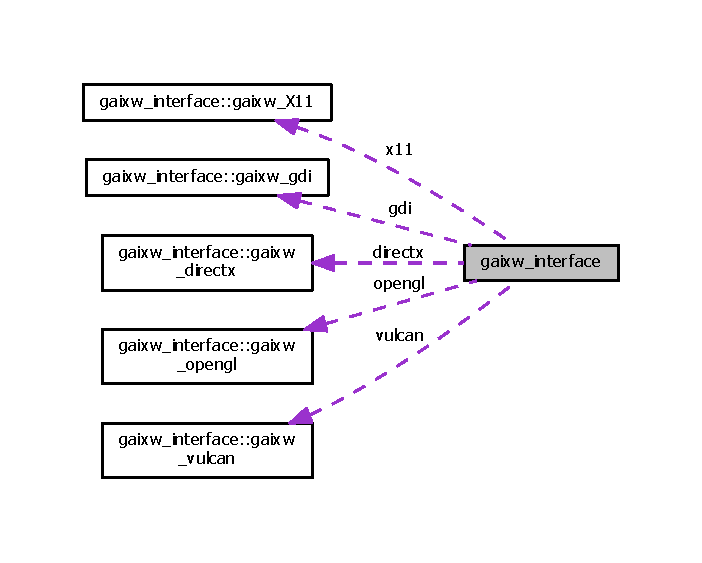
\includegraphics[width=232pt]{uniongaixw__interface__coll__graph}
\end{center}
\end{figure}
\begin{DoxyFields}{Class Members}
\mbox{\Hypertarget{gai__xwindow_8h_a639ebccdba9bbeae0d50385f08af00fa}\label{gai__xwindow_8h_a639ebccdba9bbeae0d50385f08af00fa}} 
\hyperlink{gai__xwindow_8h_structgaixw__directx}{gaixw\_directx}&
directx&
\\
\hline

\mbox{\Hypertarget{gai__xwindow_8h_a0d31586255263aeceaecba8960a37c3b}\label{gai__xwindow_8h_a0d31586255263aeceaecba8960a37c3b}} 
\hyperlink{gai__xwindow_8h_structgaixw__opengl}{gaixw\_opengl}&
opengl&
Open\+GL renderer informations like vendor, version, renderer, shading language version \\
\hline

\end{DoxyFields}
\index{gaixw\+\_\+platform\+\_\+win32@{gaixw\+\_\+platform\+\_\+win32}}\label{structgaixw__platform__win32}
\Hypertarget{gai__xwindow_8h_structgaixw__platform__win32}
\subsubsection{struct gaixw\+\_\+platform\+\_\+win32}
\begin{DoxyFields}{Class Members}
\mbox{\Hypertarget{gai__xwindow_8h_aa9da15d620888c2aa953804a90460666}\label{gai__xwindow_8h_aa9da15d620888c2aa953804a90460666}} 
HDC&
hdc&
\\
\hline

\mbox{\Hypertarget{gai__xwindow_8h_a7865b60b19703f32b629ea9c72284526}\label{gai__xwindow_8h_a7865b60b19703f32b629ea9c72284526}} 
HWND&
hwnd&
\\
\hline

\mbox{\Hypertarget{gai__xwindow_8h_a5af56cd499bebac30d7755a639670641}\label{gai__xwindow_8h_a5af56cd499bebac30d7755a639670641}} 
HINSTANCE&
instance&
\\
\hline

\mbox{\Hypertarget{gai__xwindow_8h_aa76dcd2345644ce0ea58b99954657736}\label{gai__xwindow_8h_aa76dcd2345644ce0ea58b99954657736}} 
WINDOWPLACEMENT&
position&
\\
\hline

\end{DoxyFields}
\index{gaixw\+\_\+platform\+\_\+linux@{gaixw\+\_\+platform\+\_\+linux}}\label{structgaixw__platform__linux}
\Hypertarget{gai__xwindow_8h_structgaixw__platform__linux}
\subsubsection{struct gaixw\+\_\+platform\+\_\+linux}
\begin{DoxyFields}{Class Members}
\mbox{\Hypertarget{gai__xwindow_8h_a6c2e4c461120cc843bf28c258b02c3d7}\label{gai__xwindow_8h_a6c2e4c461120cc843bf28c258b02c3d7}} 
void $\ast$&
display&
\\
\hline

\mbox{\Hypertarget{gai__xwindow_8h_a761c1cd2540e7a06bc59ca8eeb373495}\label{gai__xwindow_8h_a761c1cd2540e7a06bc59ca8eeb373495}} 
void $\ast$&
visual&
\\
\hline

\mbox{\Hypertarget{gai__xwindow_8h_af09643fe9af611052aef9d98865473ca}\label{gai__xwindow_8h_af09643fe9af611052aef9d98865473ca}} 
void $\ast$&
window&
\\
\hline

\end{DoxyFields}
\index{gaixw\+\_\+platform@{gaixw\+\_\+platform}}\label{uniongaixw__platform}
\Hypertarget{gai__xwindow_8h_uniongaixw__platform}
\subsubsection{union gaixw\+\_\+platform}


Collaboration diagram for gaixw\+\_\+platform\+:\nopagebreak
\begin{figure}[H]
\begin{center}
\leavevmode
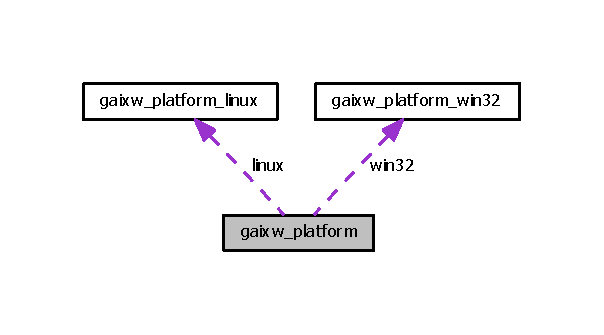
\includegraphics[width=290pt]{uniongaixw__platform__coll__graph}
\end{center}
\end{figure}
\begin{DoxyFields}{Class Members}
\mbox{\Hypertarget{gai__xwindow_8h_acd9f564fcf4c9f85b88b2a67d8e4dede}\label{gai__xwindow_8h_acd9f564fcf4c9f85b88b2a67d8e4dede}} 
\hyperlink{gai__xwindow_8h_structgaixw__platform__linux}{gaixw\_platform\_linux}&
linux&
\\
\hline

\mbox{\Hypertarget{gai__xwindow_8h_a65165dcf0ebd1548a76eb8794d12d443}\label{gai__xwindow_8h_a65165dcf0ebd1548a76eb8794d12d443}} 
\hyperlink{gai__xwindow_8h_structgaixw__platform__win32}{gaixw\_platform\_win32}&
win32&
\\
\hline

\end{DoxyFields}
\index{gaixw\+\_\+renderer@{gaixw\+\_\+renderer}}\label{structgaixw__renderer}
\Hypertarget{gai__xwindow_8h_structgaixw__renderer}
\subsubsection{struct gaixw\+\_\+renderer}


Collaboration diagram for gaixw\+\_\+renderer\+:\nopagebreak
\begin{figure}[H]
\begin{center}
\leavevmode
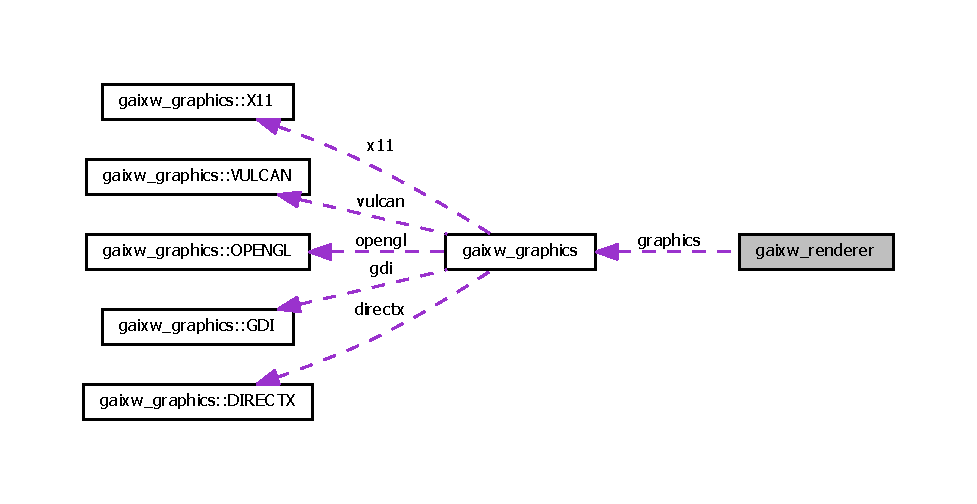
\includegraphics[width=232pt]{structgaixw__renderer__coll__graph}
\end{center}
\end{figure}
\begin{DoxyFields}{Class Members}
\mbox{\Hypertarget{gai__xwindow_8h_a201bea7ae25902eaa736de8f10556e57}\label{gai__xwindow_8h_a201bea7ae25902eaa736de8f10556e57}} 
int&
attributes&
Current state of the window. See \hyperlink{gai__xwindow_8h_a52d65318fd4fb0d358385d67f156d00c}{gaixw\+\_\+renderer\+\_\+flags} \\
\hline

\mbox{\Hypertarget{gai__xwindow_8h_a1244801c1690f8e38a1af7a5a599609f}\label{gai__xwindow_8h_a1244801c1690f8e38a1af7a5a599609f}} 
\hyperlink{gai__xwindow_8h_uniongaixw__interface}{gaixw\_interface}&
interface&
Renderer interface union for all supported renderer backends. See \hyperlink{gai__xwindow_8h_a4eae6e51f0425197a4c1010fcc7c8c9d}{gaixw\+\_\+renderer\+\_\+enum} \\
\hline

\mbox{\Hypertarget{gai__xwindow_8h_a287bd5241e45837849116cf46c5591ba}\label{gai__xwindow_8h_a287bd5241e45837849116cf46c5591ba}} 
\hyperlink{gai__xwindow_8h_a4eae6e51f0425197a4c1010fcc7c8c9d}{gaixw\_renderer\_enum}&
type&
Type of the renderer. See \hyperlink{gai__xwindow_8h_a4eae6e51f0425197a4c1010fcc7c8c9d}{gaixw\+\_\+renderer\+\_\+enum} \\
\hline

\end{DoxyFields}
\index{gaixw\+\_\+context@{gaixw\+\_\+context}}\label{structgaixw__context}
\Hypertarget{gai__xwindow_8h_structgaixw__context}
\subsubsection{struct gaixw\+\_\+context}
\begin{Desc}
\item[Examples\+: ]\par
\hyperlink{xwindow_0Cgdi_win32_0Cmain_8cpp-example}{xwindow\textbackslash{}gdi\+\_\+win32\textbackslash{}main.\+cpp}, and \hyperlink{xwindow_0Copengl_win32_0Cmain_8cpp-example}{xwindow\textbackslash{}opengl\+\_\+win32\textbackslash{}main.\+cpp}.\end{Desc}


Collaboration diagram for gaixw\+\_\+context\+:\nopagebreak
\begin{figure}[H]
\begin{center}
\leavevmode
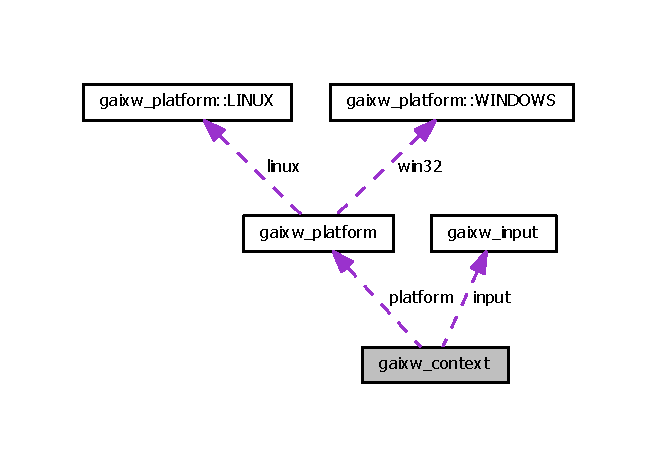
\includegraphics[width=350pt]{structgaixw__context__coll__graph}
\end{center}
\end{figure}
\begin{DoxyFields}{Class Members}
\mbox{\Hypertarget{gai__xwindow_8h_a25b8e2dded81e4335dafb70764305219}\label{gai__xwindow_8h_a25b8e2dded81e4335dafb70764305219}} 
\hyperlink{gai__xwindow_8h_structgaixw__frametime}{gaixw\_frametime}&
dt&
Time since last frame in seconds, milliseconds and microseconds \\
\hline

\mbox{\Hypertarget{gai__xwindow_8h_a488c7d5344206e2f55cd62ffc258e77b}\label{gai__xwindow_8h_a488c7d5344206e2f55cd62ffc258e77b}} 
\hyperlink{gai__xwindow_8h_structgaixw__info}{gaixw\_info}&
info&
Window information like title, width, height, x, y ... \\
\hline

\mbox{\Hypertarget{gai__xwindow_8h_a4a9d2e14ebb24977fb5df84d361c851f}\label{gai__xwindow_8h_a4a9d2e14ebb24977fb5df84d361c851f}} 
\hyperlink{gai__xwindow_8h_structgaixw__input}{gaixw\_input}&
input&
Input states for mouse and keyboard \\
\hline

\mbox{\Hypertarget{gai__xwindow_8h_a7165f8e7f0c548dd3a11c8648fb8071a}\label{gai__xwindow_8h_a7165f8e7f0c548dd3a11c8648fb8071a}} 
int&
is\_running&
Running state of the window. If the window gets closed this value will be 0. \\
\hline

\mbox{\Hypertarget{gai__xwindow_8h_acb9eb436a1a802598abfbf6934c4d8d2}\label{gai__xwindow_8h_acb9eb436a1a802598abfbf6934c4d8d2}} 
int&
is\_visible&
\\
\hline

\mbox{\Hypertarget{gai__xwindow_8h_aa297ac21e147f4cde74e021b62b3e673}\label{gai__xwindow_8h_aa297ac21e147f4cde74e021b62b3e673}} 
\hyperlink{gai__xwindow_8h_uniongaixw__platform}{gaixw\_platform}&
platform&
Platform layer union for all supported platforms \\
\hline

\mbox{\Hypertarget{gai__xwindow_8h_a5984d461e227d9028db4d9327bc9c2c4}\label{gai__xwindow_8h_a5984d461e227d9028db4d9327bc9c2c4}} 
\hyperlink{gai__xwindow_8h_structgaixw__renderer}{gaixw\_renderer}&
renderer&
Renderer struct with the current render interface \\
\hline

\end{DoxyFields}


\subsection{Macro Definition Documentation}
\mbox{\Hypertarget{gai__xwindow_8h_ab2663b30ef0369cf059d79977b93807f}\label{gai__xwindow_8h_ab2663b30ef0369cf059d79977b93807f}} 
\index{gai\+\_\+xwindow.\+h@{gai\+\_\+xwindow.\+h}!G\+A\+I\+X\+W\+\_\+\+A\+S\+S\+E\+RT@{G\+A\+I\+X\+W\+\_\+\+A\+S\+S\+E\+RT}}
\index{G\+A\+I\+X\+W\+\_\+\+A\+S\+S\+E\+RT@{G\+A\+I\+X\+W\+\_\+\+A\+S\+S\+E\+RT}!gai\+\_\+xwindow.\+h@{gai\+\_\+xwindow.\+h}}
\subsubsection{\texorpdfstring{G\+A\+I\+X\+W\+\_\+\+A\+S\+S\+E\+RT}{GAIXW\_ASSERT}}
{\footnotesize\ttfamily \#define G\+A\+I\+X\+W\+\_\+\+A\+S\+S\+E\+RT(\begin{DoxyParamCaption}\item[{}]{cond }\end{DoxyParamCaption})~assert(cond)}



Define {\bfseries G\+A\+I\+X\+W\+\_\+\+A\+S\+S\+E\+RT} before including this file to {\bfseries disable} assertions. 

\begin{DoxyNote}{Note}
Uses assert() from the c-\/standard library by default $<$assert.\+h$>$ 
\end{DoxyNote}

\begin{DoxyParams}{Parameters}
{\em cond} & Assertion condition \\
\hline
\end{DoxyParams}
\mbox{\Hypertarget{gai__xwindow_8h_aaa1d25d5e0f693faca8ccb08cc744fb6}\label{gai__xwindow_8h_aaa1d25d5e0f693faca8ccb08cc744fb6}} 
\index{gai\+\_\+xwindow.\+h@{gai\+\_\+xwindow.\+h}!G\+A\+I\+X\+W\+\_\+\+C\+L\+A\+S\+S\+N\+A\+ME@{G\+A\+I\+X\+W\+\_\+\+C\+L\+A\+S\+S\+N\+A\+ME}}
\index{G\+A\+I\+X\+W\+\_\+\+C\+L\+A\+S\+S\+N\+A\+ME@{G\+A\+I\+X\+W\+\_\+\+C\+L\+A\+S\+S\+N\+A\+ME}!gai\+\_\+xwindow.\+h@{gai\+\_\+xwindow.\+h}}
\subsubsection{\texorpdfstring{G\+A\+I\+X\+W\+\_\+\+C\+L\+A\+S\+S\+N\+A\+ME}{GAIXW\_CLASSNAME}}
{\footnotesize\ttfamily \#define G\+A\+I\+X\+W\+\_\+\+C\+L\+A\+S\+S\+N\+A\+ME~\char`\"{}libgai\+\_\+xwindow\+\_\+framework\char`\"{}}

Default classname \mbox{\Hypertarget{gai__xwindow_8h_ad52cbaf070ae26059c515d4613a401f4}\label{gai__xwindow_8h_ad52cbaf070ae26059c515d4613a401f4}} 
\index{gai\+\_\+xwindow.\+h@{gai\+\_\+xwindow.\+h}!G\+A\+I\+X\+W\+\_\+\+P\+R\+I\+NT@{G\+A\+I\+X\+W\+\_\+\+P\+R\+I\+NT}}
\index{G\+A\+I\+X\+W\+\_\+\+P\+R\+I\+NT@{G\+A\+I\+X\+W\+\_\+\+P\+R\+I\+NT}!gai\+\_\+xwindow.\+h@{gai\+\_\+xwindow.\+h}}
\subsubsection{\texorpdfstring{G\+A\+I\+X\+W\+\_\+\+P\+R\+I\+NT}{GAIXW\_PRINT}}
{\footnotesize\ttfamily \#define G\+A\+I\+X\+W\+\_\+\+P\+R\+I\+NT(\begin{DoxyParamCaption}\item[{}]{fmt,  }\item[{}]{... }\end{DoxyParamCaption})}



Define this macro before including this file if you want to redirect the output. 

Default output is set to console. (printf)

{\bfseries Example} (redirect output to Output\+Debug\+StringA on windows) 
\begin{DoxyCode}
\textcolor{keyword}{static} \textcolor{keywordtype}{char} GlobalDebugBuffer[4096];
\textcolor{preprocessor}{#define GAIXW\_PRINT(fmt, ...) snprintf(GlobalDebugBuffer, 4095, fmt, \_\_VA\_ARGS\_\_);
       OutputDebugStringA(GlobalDebugBuffer)}
\textcolor{preprocessor}{#define GAIXW\_IMPLEMENTATION}
\textcolor{preprocessor}{#include <gai\_xwindow.h>}
\end{DoxyCode}
 
\begin{DoxyParams}{Parameters}
{\em fmt} & The format \\
\hline
{\em ...} & Dynamic parameters (\+\_\+\+\_\+\+V\+A\+\_\+\+A\+R\+G\+S\+\_\+\+\_\+) \\
\hline
\end{DoxyParams}


\subsection{Enumeration Type Documentation}
\mbox{\Hypertarget{gai__xwindow_8h_a4eae6e51f0425197a4c1010fcc7c8c9d}\label{gai__xwindow_8h_a4eae6e51f0425197a4c1010fcc7c8c9d}} 
\index{gai\+\_\+xwindow.\+h@{gai\+\_\+xwindow.\+h}!gaixw\+\_\+renderer\+\_\+enum@{gaixw\+\_\+renderer\+\_\+enum}}
\index{gaixw\+\_\+renderer\+\_\+enum@{gaixw\+\_\+renderer\+\_\+enum}!gai\+\_\+xwindow.\+h@{gai\+\_\+xwindow.\+h}}
\subsubsection{\texorpdfstring{gaixw\+\_\+renderer\+\_\+enum}{gaixw\_renderer\_enum}}
{\footnotesize\ttfamily enum \hyperlink{gai__xwindow_8h_a4eae6e51f0425197a4c1010fcc7c8c9d}{gaixw\+\_\+renderer\+\_\+enum}}



Renderer backend types. 

To specifiy which backend you want to use, you have to request them like shown below.

Also see the checkout the example code section. \begin{DoxyEnumFields}{Enumerator}
\raisebox{\heightof{T}}[0pt][0pt]{\index{gaixw\+Renderer\+Unknown@{gaixw\+Renderer\+Unknown}!gai\+\_\+xwindow.\+h@{gai\+\_\+xwindow.\+h}}\index{gai\+\_\+xwindow.\+h@{gai\+\_\+xwindow.\+h}!gaixw\+Renderer\+Unknown@{gaixw\+Renderer\+Unknown}}}\mbox{\Hypertarget{gai__xwindow_8h_a4eae6e51f0425197a4c1010fcc7c8c9da25a9a692888d86fd6bf5f24e0c31a8e8}\label{gai__xwindow_8h_a4eae6e51f0425197a4c1010fcc7c8c9da25a9a692888d86fd6bf5f24e0c31a8e8}} 
gaixw\+Renderer\+Unknown&Unknown renderer type \\
\hline

\raisebox{\heightof{T}}[0pt][0pt]{\index{gaixw\+Renderer\+X11@{gaixw\+Renderer\+X11}!gai\+\_\+xwindow.\+h@{gai\+\_\+xwindow.\+h}}\index{gai\+\_\+xwindow.\+h@{gai\+\_\+xwindow.\+h}!gaixw\+Renderer\+X11@{gaixw\+Renderer\+X11}}}\mbox{\Hypertarget{gai__xwindow_8h_a4eae6e51f0425197a4c1010fcc7c8c9da2ecf0eac74bd3c8d842991bd7c0e15a0}\label{gai__xwindow_8h_a4eae6e51f0425197a4c1010fcc7c8c9da2ecf0eac74bd3c8d842991bd7c0e15a0}} 
gaixw\+Renderer\+X11&Request a X11 renderer backend \begin{DoxyNote}{Note}
Default on linux platform 
\end{DoxyNote}
\\
\hline

\raisebox{\heightof{T}}[0pt][0pt]{\index{gaixw\+Renderer\+G\+DI@{gaixw\+Renderer\+G\+DI}!gai\+\_\+xwindow.\+h@{gai\+\_\+xwindow.\+h}}\index{gai\+\_\+xwindow.\+h@{gai\+\_\+xwindow.\+h}!gaixw\+Renderer\+G\+DI@{gaixw\+Renderer\+G\+DI}}}\mbox{\Hypertarget{gai__xwindow_8h_a4eae6e51f0425197a4c1010fcc7c8c9dab382f06ccd349a4749bfcea4fd5f3080}\label{gai__xwindow_8h_a4eae6e51f0425197a4c1010fcc7c8c9dab382f06ccd349a4749bfcea4fd5f3080}} 
gaixw\+Renderer\+G\+DI&Request a G\+DI renderer backend \begin{DoxyNote}{Note}
Default on windows platform 
\end{DoxyNote}
\\
\hline

\raisebox{\heightof{T}}[0pt][0pt]{\index{gaixw\+Renderer\+D\+X10@{gaixw\+Renderer\+D\+X10}!gai\+\_\+xwindow.\+h@{gai\+\_\+xwindow.\+h}}\index{gai\+\_\+xwindow.\+h@{gai\+\_\+xwindow.\+h}!gaixw\+Renderer\+D\+X10@{gaixw\+Renderer\+D\+X10}}}\mbox{\Hypertarget{gai__xwindow_8h_a4eae6e51f0425197a4c1010fcc7c8c9da1217be504c773ce47ba76be4ddf9489d}\label{gai__xwindow_8h_a4eae6e51f0425197a4c1010fcc7c8c9da1217be504c773ce47ba76be4ddf9489d}} 
gaixw\+Renderer\+D\+X10&Request a {\bfseries DirectX} 10 renderer backend \begin{DoxyAttention}{Attention}
$\ast$$\ast$ N\+OT I\+M\+P\+L\+E\+M\+E\+N\+T\+ED Y\+ET $\ast$$\ast$ 
\end{DoxyAttention}
\\
\hline

\raisebox{\heightof{T}}[0pt][0pt]{\index{gaixw\+Renderer\+D\+X11@{gaixw\+Renderer\+D\+X11}!gai\+\_\+xwindow.\+h@{gai\+\_\+xwindow.\+h}}\index{gai\+\_\+xwindow.\+h@{gai\+\_\+xwindow.\+h}!gaixw\+Renderer\+D\+X11@{gaixw\+Renderer\+D\+X11}}}\mbox{\Hypertarget{gai__xwindow_8h_a4eae6e51f0425197a4c1010fcc7c8c9dab19a6d88f34235d7333fbc209d1f178a}\label{gai__xwindow_8h_a4eae6e51f0425197a4c1010fcc7c8c9dab19a6d88f34235d7333fbc209d1f178a}} 
gaixw\+Renderer\+D\+X11&Request a {\bfseries DirectX} 11 renderer backend \begin{DoxyAttention}{Attention}
$\ast$$\ast$ N\+OT I\+M\+P\+L\+E\+M\+E\+N\+T\+ED Y\+ET $\ast$$\ast$ 
\end{DoxyAttention}
\\
\hline

\raisebox{\heightof{T}}[0pt][0pt]{\index{gaixw\+Renderer\+D\+X12@{gaixw\+Renderer\+D\+X12}!gai\+\_\+xwindow.\+h@{gai\+\_\+xwindow.\+h}}\index{gai\+\_\+xwindow.\+h@{gai\+\_\+xwindow.\+h}!gaixw\+Renderer\+D\+X12@{gaixw\+Renderer\+D\+X12}}}\mbox{\Hypertarget{gai__xwindow_8h_a4eae6e51f0425197a4c1010fcc7c8c9da8cd168a752459bca73bdea7b77eb421e}\label{gai__xwindow_8h_a4eae6e51f0425197a4c1010fcc7c8c9da8cd168a752459bca73bdea7b77eb421e}} 
gaixw\+Renderer\+D\+X12&Request a {\bfseries DirectX} 12 renderer backend \begin{DoxyAttention}{Attention}
$\ast$$\ast$ N\+OT I\+M\+P\+L\+E\+M\+E\+N\+T\+ED Y\+ET $\ast$$\ast$ 
\end{DoxyAttention}
\\
\hline

\raisebox{\heightof{T}}[0pt][0pt]{\index{gaixw\+Renderer\+Open\+GL@{gaixw\+Renderer\+Open\+GL}!gai\+\_\+xwindow.\+h@{gai\+\_\+xwindow.\+h}}\index{gai\+\_\+xwindow.\+h@{gai\+\_\+xwindow.\+h}!gaixw\+Renderer\+Open\+GL@{gaixw\+Renderer\+Open\+GL}}}\mbox{\Hypertarget{gai__xwindow_8h_a4eae6e51f0425197a4c1010fcc7c8c9daf43570fcfedb502e88eb5c69f0eeecc1}\label{gai__xwindow_8h_a4eae6e51f0425197a4c1010fcc7c8c9daf43570fcfedb502e88eb5c69f0eeecc1}} 
gaixw\+Renderer\+Open\+GL&Request an {\bfseries Open\+GL} renderer backend


\begin{DoxyCode}
\textcolor{preprocessor}{#define GAIXW\_OPENGL}
\textcolor{preprocessor}{#define GAIXW\_OPENGL\_MAJOR 4            // Optional macro! Not needed if you dont want to specify this.}
\textcolor{preprocessor}{#define GAIXW\_OPENGL\_MINOR 3            // Optional macro! Not needed if you dont want to specify this.}
\textcolor{preprocessor}{#define GAIXW\_IMPLEMENTATION}
\textcolor{preprocessor}{#include <gai\_xwindow.h>}
\end{DoxyCode}


\begin{DoxyNote}{Note}
You can also request a modern opengl context (3.\+x or higher) 
\end{DoxyNote}
\\
\hline

\raisebox{\heightof{T}}[0pt][0pt]{\index{gaixw\+Renderer\+Vulcan@{gaixw\+Renderer\+Vulcan}!gai\+\_\+xwindow.\+h@{gai\+\_\+xwindow.\+h}}\index{gai\+\_\+xwindow.\+h@{gai\+\_\+xwindow.\+h}!gaixw\+Renderer\+Vulcan@{gaixw\+Renderer\+Vulcan}}}\mbox{\Hypertarget{gai__xwindow_8h_a4eae6e51f0425197a4c1010fcc7c8c9da4cd9efc9b0b4bcc5674423557a0214ab}\label{gai__xwindow_8h_a4eae6e51f0425197a4c1010fcc7c8c9da4cd9efc9b0b4bcc5674423557a0214ab}} 
gaixw\+Renderer\+Vulcan&Request a {\bfseries vulcan} renderer backend \begin{DoxyAttention}{Attention}
$\ast$$\ast$ N\+OT I\+M\+P\+L\+E\+M\+E\+N\+T\+ED Y\+ET $\ast$$\ast$ 
\end{DoxyAttention}
\\
\hline

\end{DoxyEnumFields}
\mbox{\Hypertarget{gai__xwindow_8h_a52d65318fd4fb0d358385d67f156d00c}\label{gai__xwindow_8h_a52d65318fd4fb0d358385d67f156d00c}} 
\index{gai\+\_\+xwindow.\+h@{gai\+\_\+xwindow.\+h}!gaixw\+\_\+renderer\+\_\+flags@{gaixw\+\_\+renderer\+\_\+flags}}
\index{gaixw\+\_\+renderer\+\_\+flags@{gaixw\+\_\+renderer\+\_\+flags}!gai\+\_\+xwindow.\+h@{gai\+\_\+xwindow.\+h}}
\subsubsection{\texorpdfstring{gaixw\+\_\+renderer\+\_\+flags}{gaixw\_renderer\_flags}}
{\footnotesize\ttfamily enum \hyperlink{gai__xwindow_8h_a52d65318fd4fb0d358385d67f156d00c}{gaixw\+\_\+renderer\+\_\+flags}}



Renderer flags. 

\begin{DoxyEnumFields}{Enumerator}
\raisebox{\heightof{T}}[0pt][0pt]{\index{gaixw\+Flags\+Minimized@{gaixw\+Flags\+Minimized}!gai\+\_\+xwindow.\+h@{gai\+\_\+xwindow.\+h}}\index{gai\+\_\+xwindow.\+h@{gai\+\_\+xwindow.\+h}!gaixw\+Flags\+Minimized@{gaixw\+Flags\+Minimized}}}\mbox{\Hypertarget{gai__xwindow_8h_a52d65318fd4fb0d358385d67f156d00ca024bb28b1d09e6dabb43cca1db088cd1}\label{gai__xwindow_8h_a52d65318fd4fb0d358385d67f156d00ca024bb28b1d09e6dabb43cca1db088cd1}} 
gaixw\+Flags\+Minimized&Window is minimized \\
\hline

\raisebox{\heightof{T}}[0pt][0pt]{\index{gaixw\+Flags\+Maximized@{gaixw\+Flags\+Maximized}!gai\+\_\+xwindow.\+h@{gai\+\_\+xwindow.\+h}}\index{gai\+\_\+xwindow.\+h@{gai\+\_\+xwindow.\+h}!gaixw\+Flags\+Maximized@{gaixw\+Flags\+Maximized}}}\mbox{\Hypertarget{gai__xwindow_8h_a52d65318fd4fb0d358385d67f156d00ca4c1b948394dbf097f6007e01ded11242}\label{gai__xwindow_8h_a52d65318fd4fb0d358385d67f156d00ca4c1b948394dbf097f6007e01ded11242}} 
gaixw\+Flags\+Maximized&Window is maximized \\
\hline

\raisebox{\heightof{T}}[0pt][0pt]{\index{gaixw\+Flags\+Fullscreen@{gaixw\+Flags\+Fullscreen}!gai\+\_\+xwindow.\+h@{gai\+\_\+xwindow.\+h}}\index{gai\+\_\+xwindow.\+h@{gai\+\_\+xwindow.\+h}!gaixw\+Flags\+Fullscreen@{gaixw\+Flags\+Fullscreen}}}\mbox{\Hypertarget{gai__xwindow_8h_a52d65318fd4fb0d358385d67f156d00ca1b5d286481622b104b8dd24bf3114cd2}\label{gai__xwindow_8h_a52d65318fd4fb0d358385d67f156d00ca1b5d286481622b104b8dd24bf3114cd2}} 
gaixw\+Flags\+Fullscreen&Window is in fullscreen mode \\
\hline

\raisebox{\heightof{T}}[0pt][0pt]{\index{gaixw\+Flags\+V\+S\+Y\+NC@{gaixw\+Flags\+V\+S\+Y\+NC}!gai\+\_\+xwindow.\+h@{gai\+\_\+xwindow.\+h}}\index{gai\+\_\+xwindow.\+h@{gai\+\_\+xwindow.\+h}!gaixw\+Flags\+V\+S\+Y\+NC@{gaixw\+Flags\+V\+S\+Y\+NC}}}\mbox{\Hypertarget{gai__xwindow_8h_a52d65318fd4fb0d358385d67f156d00ca39f9d8a5253caf225480a80d1b52e4c2}\label{gai__xwindow_8h_a52d65318fd4fb0d358385d67f156d00ca39f9d8a5253caf225480a80d1b52e4c2}} 
gaixw\+Flags\+V\+S\+Y\+NC&Window has vertical sync enabled \\
\hline

\end{DoxyEnumFields}


\subsection{Function Documentation}
\mbox{\Hypertarget{gai__xwindow_8h_a986353262ac6038b69005bec8111ac56}\label{gai__xwindow_8h_a986353262ac6038b69005bec8111ac56}} 
\index{gai\+\_\+xwindow.\+h@{gai\+\_\+xwindow.\+h}!gaixw\+\_\+\+Deinit@{gaixw\+\_\+\+Deinit}}
\index{gaixw\+\_\+\+Deinit@{gaixw\+\_\+\+Deinit}!gai\+\_\+xwindow.\+h@{gai\+\_\+xwindow.\+h}}
\subsubsection{\texorpdfstring{gaixw\+\_\+\+Deinit()}{gaixw\_Deinit()}}
{\footnotesize\ttfamily \hyperlink{gai__xwindow_8h_ab41ae714bb16012af56329f9032e6d16}{G\+A\+I\+X\+W\+\_\+\+A\+PI} void gaixw\+\_\+\+Deinit (\begin{DoxyParamCaption}\item[{\hyperlink{gai__xwindow_8h_structgaixw__context}{gaixw\+\_\+context} $\ast$}]{window }\end{DoxyParamCaption})}



Deinitializes the window. 


\begin{DoxyParams}{Parameters}
{\em window} & A pointer to a \hyperlink{gai__xwindow_8h_structgaixw__context}{gaixw\+\_\+context} structure \\
\hline
\end{DoxyParams}
\begin{Desc}
\item[Examples\+: ]\par
\hyperlink{xwindow_0Cgdi_win32_0Cmain_8cpp-example}{xwindow\textbackslash{}gdi\+\_\+win32\textbackslash{}main.\+cpp}, and \hyperlink{xwindow_0Copengl_win32_0Cmain_8cpp-example}{xwindow\textbackslash{}opengl\+\_\+win32\textbackslash{}main.\+cpp}.\end{Desc}
\mbox{\Hypertarget{gai__xwindow_8h_a11552275ad444bc3be3b6a5a5b214c7d}\label{gai__xwindow_8h_a11552275ad444bc3be3b6a5a5b214c7d}} 
\index{gai\+\_\+xwindow.\+h@{gai\+\_\+xwindow.\+h}!gaixw\+\_\+\+Get\+Attribute@{gaixw\+\_\+\+Get\+Attribute}}
\index{gaixw\+\_\+\+Get\+Attribute@{gaixw\+\_\+\+Get\+Attribute}!gai\+\_\+xwindow.\+h@{gai\+\_\+xwindow.\+h}}
\subsubsection{\texorpdfstring{gaixw\+\_\+\+Get\+Attribute()}{gaixw\_GetAttribute()}}
{\footnotesize\ttfamily \hyperlink{gai__xwindow_8h_ab41ae714bb16012af56329f9032e6d16}{G\+A\+I\+X\+W\+\_\+\+A\+PI} unsigned int gaixw\+\_\+\+Get\+Attribute (\begin{DoxyParamCaption}\item[{\hyperlink{gai__xwindow_8h_structgaixw__context}{gaixw\+\_\+context} $\ast$}]{window,  }\item[{\hyperlink{gai__xwindow_8h_a52d65318fd4fb0d358385d67f156d00c}{gaixw\+\_\+renderer\+\_\+flags}}]{attrib }\end{DoxyParamCaption})}



Current attribute state of the window. 


\begin{DoxyParams}{Parameters}
{\em window} & A pointer to a \hyperlink{gai__xwindow_8h_structgaixw__context}{gaixw\+\_\+context} structure \\
\hline
{\em attrib} & Attribute flags as specified in \hyperlink{gai__xwindow_8h_a52d65318fd4fb0d358385d67f156d00c}{gaixw\+\_\+renderer\+\_\+flags}~\newline
\hyperlink{gai__xwindow_8h_a52d65318fd4fb0d358385d67f156d00ca024bb28b1d09e6dabb43cca1db088cd1}{gaixw\+Flags\+Minimized}~\newline
\hyperlink{gai__xwindow_8h_a52d65318fd4fb0d358385d67f156d00ca4c1b948394dbf097f6007e01ded11242}{gaixw\+Flags\+Maximized}~\newline
\hyperlink{gai__xwindow_8h_a52d65318fd4fb0d358385d67f156d00ca1b5d286481622b104b8dd24bf3114cd2}{gaixw\+Flags\+Fullscreen}~\newline
\hyperlink{gai__xwindow_8h_a52d65318fd4fb0d358385d67f156d00ca39f9d8a5253caf225480a80d1b52e4c2}{gaixw\+Flags\+V\+S\+Y\+NC}~\newline
 \\
\hline
\end{DoxyParams}
\begin{DoxyReturn}{Returns}
\tabulinesep=1mm
\begin{longtabu} spread 0pt [c]{*{2}{|X[-1]}|}
\hline
\rowcolor{\tableheadbgcolor}\textbf{ Return Code }&\textbf{ Description  }\\\cline{1-2}
\endfirsthead
\hline
\endfoot
\hline
\rowcolor{\tableheadbgcolor}\textbf{ Return Code }&\textbf{ Description  }\\\cline{1-2}
\endhead
1 &Set \\\cline{1-2}
0 &Not set \\\cline{1-2}
\end{longtabu}

\end{DoxyReturn}
\mbox{\Hypertarget{gai__xwindow_8h_afb8573bf3e47bef617b0c575cabd56b1}\label{gai__xwindow_8h_afb8573bf3e47bef617b0c575cabd56b1}} 
\index{gai\+\_\+xwindow.\+h@{gai\+\_\+xwindow.\+h}!gaixw\+\_\+\+Get\+Proc@{gaixw\+\_\+\+Get\+Proc}}
\index{gaixw\+\_\+\+Get\+Proc@{gaixw\+\_\+\+Get\+Proc}!gai\+\_\+xwindow.\+h@{gai\+\_\+xwindow.\+h}}
\subsubsection{\texorpdfstring{gaixw\+\_\+\+Get\+Proc()}{gaixw\_GetProc()}}
{\footnotesize\ttfamily \hyperlink{gai__xwindow_8h_ab41ae714bb16012af56329f9032e6d16}{G\+A\+I\+X\+W\+\_\+\+A\+PI} void$\ast$ gaixw\+\_\+\+Get\+Proc (\begin{DoxyParamCaption}\item[{\hyperlink{gai__xwindow_8h_structgaixw__context}{gaixw\+\_\+context} $\ast$}]{window,  }\item[{const char $\ast$}]{name }\end{DoxyParamCaption})}



Gets the procedure\textquotesingle{}s memory address for the specified function name. 


\begin{DoxyParams}{Parameters}
{\em window} & A pointer to a \hyperlink{gai__xwindow_8h_structgaixw__context}{gaixw\+\_\+context} structure \\
\hline
{\em name} & Name of the function\\
\hline
\end{DoxyParams}
\begin{DoxyReturn}{Returns}
\tabulinesep=1mm
\begin{longtabu} spread 0pt [c]{*{2}{|X[-1]}|}
\hline
\rowcolor{\tableheadbgcolor}\textbf{ Return Code }&\textbf{ Description  }\\\cline{1-2}
\endfirsthead
\hline
\endfoot
\hline
\rowcolor{\tableheadbgcolor}\textbf{ Return Code }&\textbf{ Description  }\\\cline{1-2}
\endhead
0 &Null ( function with that name not found ) \\\cline{1-2}
Pointer &A pointer to functions address \\\cline{1-2}
\end{longtabu}

\end{DoxyReturn}
\mbox{\Hypertarget{gai__xwindow_8h_a47de27dee38c387b49ac60e21b6b27af}\label{gai__xwindow_8h_a47de27dee38c387b49ac60e21b6b27af}} 
\index{gai\+\_\+xwindow.\+h@{gai\+\_\+xwindow.\+h}!gaixw\+\_\+\+Hide@{gaixw\+\_\+\+Hide}}
\index{gaixw\+\_\+\+Hide@{gaixw\+\_\+\+Hide}!gai\+\_\+xwindow.\+h@{gai\+\_\+xwindow.\+h}}
\subsubsection{\texorpdfstring{gaixw\+\_\+\+Hide()}{gaixw\_Hide()}}
{\footnotesize\ttfamily \hyperlink{gai__xwindow_8h_ab41ae714bb16012af56329f9032e6d16}{G\+A\+I\+X\+W\+\_\+\+A\+PI} int gaixw\+\_\+\+Hide (\begin{DoxyParamCaption}\item[{\hyperlink{gai__xwindow_8h_structgaixw__context}{gaixw\+\_\+context} $\ast$}]{window }\end{DoxyParamCaption})}



Hides the window from the user. 


\begin{DoxyParams}{Parameters}
{\em window} & A pointer to a \hyperlink{gai__xwindow_8h_structgaixw__context}{gaixw\+\_\+context} structure\\
\hline
\end{DoxyParams}
\begin{DoxyReturn}{Returns}
\tabulinesep=1mm
\begin{longtabu} spread 0pt [c]{*{2}{|X[-1]}|}
\hline
\rowcolor{\tableheadbgcolor}\textbf{ Return Code }&\textbf{ Description  }\\\cline{1-2}
\endfirsthead
\hline
\endfoot
\hline
\rowcolor{\tableheadbgcolor}\textbf{ Return Code }&\textbf{ Description  }\\\cline{1-2}
\endhead
1 &Success \\\cline{1-2}
0 &Failure \\\cline{1-2}
\end{longtabu}

\end{DoxyReturn}
\mbox{\Hypertarget{gai__xwindow_8h_adec8bb998b6861c4d239b25634c8eb55}\label{gai__xwindow_8h_adec8bb998b6861c4d239b25634c8eb55}} 
\index{gai\+\_\+xwindow.\+h@{gai\+\_\+xwindow.\+h}!gaixw\+\_\+\+Init@{gaixw\+\_\+\+Init}}
\index{gaixw\+\_\+\+Init@{gaixw\+\_\+\+Init}!gai\+\_\+xwindow.\+h@{gai\+\_\+xwindow.\+h}}
\subsubsection{\texorpdfstring{gaixw\+\_\+\+Init()}{gaixw\_Init()}}
{\footnotesize\ttfamily \hyperlink{gai__xwindow_8h_ab41ae714bb16012af56329f9032e6d16}{G\+A\+I\+X\+W\+\_\+\+A\+PI} int gaixw\+\_\+\+Init (\begin{DoxyParamCaption}\item[{\hyperlink{gai__xwindow_8h_structgaixw__context}{gaixw\+\_\+context} $\ast$}]{window,  }\item[{const char $\ast$}]{title = {\ttfamily \char`\"{}default~window~title\char`\"{}},  }\item[{int}]{width = {\ttfamily -\/1},  }\item[{int}]{height = {\ttfamily -\/1},  }\item[{int}]{x = {\ttfamily -\/1},  }\item[{int}]{y = {\ttfamily -\/1},  }\item[{const char $\ast$}]{classname = {\ttfamily \hyperlink{gai__xwindow_8h_aaa1d25d5e0f693faca8ccb08cc744fb6}{G\+A\+I\+X\+W\+\_\+\+C\+L\+A\+S\+S\+N\+A\+ME}},  }\item[{unsigned int}]{visible = {\ttfamily 1} }\end{DoxyParamCaption})}



Initializes a window for the current platform. 


\begin{DoxyParams}{Parameters}
{\em window} & A pointer to a \hyperlink{gai__xwindow_8h_structgaixw__context}{gaixw\+\_\+context} structure \\
\hline
{\em title} & (optional) Title \\
\hline
{\em width} & (optional) Width \\
\hline
{\em height} & (optional) Height \\
\hline
{\em x} & (optional) X position \\
\hline
{\em y} & (optional) Y position \\
\hline
{\em classname} & (optional) Unique classname for this window instance \\
\hline
{\em visible} & (optional) Specifies if the window is visible after creation or not\\
\hline
\end{DoxyParams}
\begin{DoxyReturn}{Returns}
\tabulinesep=1mm
\begin{longtabu} spread 0pt [c]{*{3}{|X[-1]}|}
\hline
\rowcolor{\tableheadbgcolor}\textbf{ Returns }&\textbf{ Windows }&\textbf{ Linux  }\\\cline{1-3}
\endfirsthead
\hline
\endfoot
\hline
\rowcolor{\tableheadbgcolor}\textbf{ Returns }&\textbf{ Windows }&\textbf{ Linux  }\\\cline{1-3}
\endhead
1 &Success &Success \\\cline{1-3}
0 &Convert\+Thread\+To\+Fiber failed &Not implemented yet! \\\cline{1-3}
-\/1 &Register\+Class\+ExA failed &Not implemented yet! \\\cline{1-3}
-\/2 &Create\+WindowA failed &Not implemented yet! \\\cline{1-3}
-\/3 &(Open\+GL) Choose\+Pixel\+Format failed &Not implemented yet! \\\cline{1-3}
-\/4 &(Open\+GL) Set\+Pixel\+Format failed &Not implemented yet! \\\cline{1-3}
-\/5 &(Open\+GL) wgl\+Create\+Context failed &Not implemented yet! \\\cline{1-3}
-\/6 &(Open\+GL) wgl\+Make\+Current failed &Not implemented yet! \\\cline{1-3}
\end{longtabu}

\end{DoxyReturn}
{\bfseries Snippet (default gdi)\+:} 
\begin{DoxyCodeInclude}
    \textcolor{keywordtype}{int} retval = 0;
    \hyperlink{gai__xwindow_8h_structgaixw__context}{gaixw\_context} window = \{\};
    retval = \hyperlink{gai__xwindow_8h_adec8bb998b6861c4d239b25634c8eb55}{gaixw\_Init}(&window, \textcolor{stringliteral}{"gdi example"}, 640, 480);
    \textcolor{keywordflow}{if}(retval != 1) \textcolor{keywordflow}{return} retval;
\end{DoxyCodeInclude}
\begin{Desc}
\item[Examples\+: ]\par
\hyperlink{xwindow_0Cgdi_win32_0Cmain_8cpp-example}{xwindow\textbackslash{}gdi\+\_\+win32\textbackslash{}main.\+cpp}, and \hyperlink{xwindow_0Copengl_win32_0Cmain_8cpp-example}{xwindow\textbackslash{}opengl\+\_\+win32\textbackslash{}main.\+cpp}.\end{Desc}
\mbox{\Hypertarget{gai__xwindow_8h_ada33bbd9a3e4d2101a910a08ab4c3128}\label{gai__xwindow_8h_ada33bbd9a3e4d2101a910a08ab4c3128}} 
\index{gai\+\_\+xwindow.\+h@{gai\+\_\+xwindow.\+h}!gaixw\+\_\+\+Is\+Fullscreen@{gaixw\+\_\+\+Is\+Fullscreen}}
\index{gaixw\+\_\+\+Is\+Fullscreen@{gaixw\+\_\+\+Is\+Fullscreen}!gai\+\_\+xwindow.\+h@{gai\+\_\+xwindow.\+h}}
\subsubsection{\texorpdfstring{gaixw\+\_\+\+Is\+Fullscreen()}{gaixw\_IsFullscreen()}}
{\footnotesize\ttfamily \hyperlink{gai__xwindow_8h_ab41ae714bb16012af56329f9032e6d16}{G\+A\+I\+X\+W\+\_\+\+A\+PI} int gaixw\+\_\+\+Is\+Fullscreen (\begin{DoxyParamCaption}\item[{\hyperlink{gai__xwindow_8h_structgaixw__context}{gaixw\+\_\+context} $\ast$}]{window }\end{DoxyParamCaption})}



Current state of fullscreen. 


\begin{DoxyParams}{Parameters}
{\em window} & A pointer to a \hyperlink{gai__xwindow_8h_structgaixw__context}{gaixw\+\_\+context} structure\\
\hline
\end{DoxyParams}
\begin{DoxyReturn}{Returns}
\tabulinesep=1mm
\begin{longtabu} spread 0pt [c]{*{2}{|X[-1]}|}
\hline
\rowcolor{\tableheadbgcolor}\textbf{ Return Code }&\textbf{ Description  }\\\cline{1-2}
\endfirsthead
\hline
\endfoot
\hline
\rowcolor{\tableheadbgcolor}\textbf{ Return Code }&\textbf{ Description  }\\\cline{1-2}
\endhead
1 &Fullscreen enabled \\\cline{1-2}
0 &Fullscreen disabled \\\cline{1-2}
\end{longtabu}

\end{DoxyReturn}
\mbox{\Hypertarget{gai__xwindow_8h_a8bae66c5869f3d948b9f4f520fcba566}\label{gai__xwindow_8h_a8bae66c5869f3d948b9f4f520fcba566}} 
\index{gai\+\_\+xwindow.\+h@{gai\+\_\+xwindow.\+h}!gaixw\+\_\+\+Is\+Vertical\+Sync\+Enabled@{gaixw\+\_\+\+Is\+Vertical\+Sync\+Enabled}}
\index{gaixw\+\_\+\+Is\+Vertical\+Sync\+Enabled@{gaixw\+\_\+\+Is\+Vertical\+Sync\+Enabled}!gai\+\_\+xwindow.\+h@{gai\+\_\+xwindow.\+h}}
\subsubsection{\texorpdfstring{gaixw\+\_\+\+Is\+Vertical\+Sync\+Enabled()}{gaixw\_IsVerticalSyncEnabled()}}
{\footnotesize\ttfamily \hyperlink{gai__xwindow_8h_ab41ae714bb16012af56329f9032e6d16}{G\+A\+I\+X\+W\+\_\+\+A\+PI} int gaixw\+\_\+\+Is\+Vertical\+Sync\+Enabled (\begin{DoxyParamCaption}\item[{\hyperlink{gai__xwindow_8h_structgaixw__context}{gaixw\+\_\+context} $\ast$}]{window }\end{DoxyParamCaption})}



Gets the vertical sync state. 

\begin{DoxyNote}{Note}
This is a call to the graphics driver. Since the drivers implementations are different, this can have different results on different graphic cards.
\end{DoxyNote}

\begin{DoxyParams}{Parameters}
{\em window} & A pointer to a \hyperlink{gai__xwindow_8h_structgaixw__context}{gaixw\+\_\+context} structure\\
\hline
\end{DoxyParams}
\begin{DoxyReturn}{Returns}
\tabulinesep=1mm
\begin{longtabu} spread 0pt [c]{*{2}{|X[-1]}|}
\hline
\rowcolor{\tableheadbgcolor}\textbf{ Return Code }&\textbf{ Description  }\\\cline{1-2}
\endfirsthead
\hline
\endfoot
\hline
\rowcolor{\tableheadbgcolor}\textbf{ Return Code }&\textbf{ Description  }\\\cline{1-2}
\endhead
1 &V\+S\+Y\+NC enabled \\\cline{1-2}
0 &V\+S\+Y\+NC disabled \\\cline{1-2}
\end{longtabu}

\end{DoxyReturn}
\mbox{\Hypertarget{gai__xwindow_8h_ae980b54b9a83cb2babcfd1492600fc95}\label{gai__xwindow_8h_ae980b54b9a83cb2babcfd1492600fc95}} 
\index{gai\+\_\+xwindow.\+h@{gai\+\_\+xwindow.\+h}!gaixw\+\_\+\+Key\+Down@{gaixw\+\_\+\+Key\+Down}}
\index{gaixw\+\_\+\+Key\+Down@{gaixw\+\_\+\+Key\+Down}!gai\+\_\+xwindow.\+h@{gai\+\_\+xwindow.\+h}}
\subsubsection{\texorpdfstring{gaixw\+\_\+\+Key\+Down()}{gaixw\_KeyDown()}}
{\footnotesize\ttfamily \hyperlink{gai__xwindow_8h_ab41ae714bb16012af56329f9032e6d16}{G\+A\+I\+X\+W\+\_\+\+A\+PI} unsigned char gaixw\+\_\+\+Key\+Down (\begin{DoxyParamCaption}\item[{\hyperlink{gai__xwindow_8h_structgaixw__context}{gaixw\+\_\+context} $\ast$}]{window,  }\item[{int}]{key }\end{DoxyParamCaption})}



Current state of the specified keyboard key. 


\begin{DoxyParams}{Parameters}
{\em window} & A pointer to a \hyperlink{gai__xwindow_8h_structgaixw__context}{gaixw\+\_\+context} structure \\
\hline
{\em key} & Keycode between 0-\/255\\
\hline
\end{DoxyParams}
\begin{DoxyReturn}{Returns}
\tabulinesep=1mm
\begin{longtabu} spread 0pt [c]{*{2}{|X[-1]}|}
\hline
\rowcolor{\tableheadbgcolor}\textbf{ Return Code }&\textbf{ Description  }\\\cline{1-2}
\endfirsthead
\hline
\endfoot
\hline
\rowcolor{\tableheadbgcolor}\textbf{ Return Code }&\textbf{ Description  }\\\cline{1-2}
\endhead
1 &Pressed \\\cline{1-2}
0 &Not pressed \\\cline{1-2}
\end{longtabu}

\end{DoxyReturn}
\mbox{\Hypertarget{gai__xwindow_8h_a2166c011f837a9aa530d22ba2f1c5f93}\label{gai__xwindow_8h_a2166c011f837a9aa530d22ba2f1c5f93}} 
\index{gai\+\_\+xwindow.\+h@{gai\+\_\+xwindow.\+h}!gaixw\+\_\+\+Key\+Pressed@{gaixw\+\_\+\+Key\+Pressed}}
\index{gaixw\+\_\+\+Key\+Pressed@{gaixw\+\_\+\+Key\+Pressed}!gai\+\_\+xwindow.\+h@{gai\+\_\+xwindow.\+h}}
\subsubsection{\texorpdfstring{gaixw\+\_\+\+Key\+Pressed()}{gaixw\_KeyPressed()}}
{\footnotesize\ttfamily \hyperlink{gai__xwindow_8h_ab41ae714bb16012af56329f9032e6d16}{G\+A\+I\+X\+W\+\_\+\+A\+PI} unsigned char gaixw\+\_\+\+Key\+Pressed (\begin{DoxyParamCaption}\item[{\hyperlink{gai__xwindow_8h_structgaixw__context}{gaixw\+\_\+context} $\ast$}]{window,  }\item[{int}]{key }\end{DoxyParamCaption})}



Current pressed state of the specified keyboard key. 

\begin{DoxyNote}{Note}
This only returns 1 if the key was {\bfseries released} before and is now {\bfseries pressed} (Only occurs once)
\end{DoxyNote}

\begin{DoxyParams}[1]{Parameters}
 & {\em window} & A pointer to a \hyperlink{gai__xwindow_8h_structgaixw__context}{gaixw\+\_\+context} structure \\
\hline
\mbox{\tt in}  & {\em key} & Keycode between 0-\/255\\
\hline
\end{DoxyParams}
\begin{DoxyReturn}{Returns}
\tabulinesep=1mm
\begin{longtabu} spread 0pt [c]{*{2}{|X[-1]}|}
\hline
\rowcolor{\tableheadbgcolor}\textbf{ Return Code }&\textbf{ Description  }\\\cline{1-2}
\endfirsthead
\hline
\endfoot
\hline
\rowcolor{\tableheadbgcolor}\textbf{ Return Code }&\textbf{ Description  }\\\cline{1-2}
\endhead
1 &Was pressed \\\cline{1-2}
0 &Not pressed \\\cline{1-2}
\end{longtabu}

\end{DoxyReturn}
\mbox{\Hypertarget{gai__xwindow_8h_ab9d00faab4d5c7f758aa998b82ffe3fd}\label{gai__xwindow_8h_ab9d00faab4d5c7f758aa998b82ffe3fd}} 
\index{gai\+\_\+xwindow.\+h@{gai\+\_\+xwindow.\+h}!gaixw\+\_\+\+Key\+Released@{gaixw\+\_\+\+Key\+Released}}
\index{gaixw\+\_\+\+Key\+Released@{gaixw\+\_\+\+Key\+Released}!gai\+\_\+xwindow.\+h@{gai\+\_\+xwindow.\+h}}
\subsubsection{\texorpdfstring{gaixw\+\_\+\+Key\+Released()}{gaixw\_KeyReleased()}}
{\footnotesize\ttfamily \hyperlink{gai__xwindow_8h_ab41ae714bb16012af56329f9032e6d16}{G\+A\+I\+X\+W\+\_\+\+A\+PI} unsigned char gaixw\+\_\+\+Key\+Released (\begin{DoxyParamCaption}\item[{\hyperlink{gai__xwindow_8h_structgaixw__context}{gaixw\+\_\+context} $\ast$}]{window,  }\item[{int}]{key }\end{DoxyParamCaption})}



Current released state of the specified keyboard key. 

\begin{DoxyNote}{Note}
This only returns 1 if the key was {\bfseries pressed} before and is now {\bfseries released} (Only occurs once)
\end{DoxyNote}

\begin{DoxyParams}[1]{Parameters}
 & {\em window} & A pointer to a \hyperlink{gai__xwindow_8h_structgaixw__context}{gaixw\+\_\+context} structure \\
\hline
\mbox{\tt in}  & {\em key} & Keycode between 0-\/255\\
\hline
\end{DoxyParams}
\begin{DoxyReturn}{Returns}
\tabulinesep=1mm
\begin{longtabu} spread 0pt [c]{*{2}{|X[-1]}|}
\hline
\rowcolor{\tableheadbgcolor}\textbf{ Return Code }&\textbf{ Description  }\\\cline{1-2}
\endfirsthead
\hline
\endfoot
\hline
\rowcolor{\tableheadbgcolor}\textbf{ Return Code }&\textbf{ Description  }\\\cline{1-2}
\endhead
1 &Was released \\\cline{1-2}
0 &Not released \\\cline{1-2}
\end{longtabu}

\end{DoxyReturn}
\mbox{\Hypertarget{gai__xwindow_8h_ad65b54072e30a2c5b74602dc5d515b9f}\label{gai__xwindow_8h_ad65b54072e30a2c5b74602dc5d515b9f}} 
\index{gai\+\_\+xwindow.\+h@{gai\+\_\+xwindow.\+h}!gaixw\+\_\+\+Mouse\+Down@{gaixw\+\_\+\+Mouse\+Down}}
\index{gaixw\+\_\+\+Mouse\+Down@{gaixw\+\_\+\+Mouse\+Down}!gai\+\_\+xwindow.\+h@{gai\+\_\+xwindow.\+h}}
\subsubsection{\texorpdfstring{gaixw\+\_\+\+Mouse\+Down()}{gaixw\_MouseDown()}}
{\footnotesize\ttfamily \hyperlink{gai__xwindow_8h_ab41ae714bb16012af56329f9032e6d16}{G\+A\+I\+X\+W\+\_\+\+A\+PI} unsigned char gaixw\+\_\+\+Mouse\+Down (\begin{DoxyParamCaption}\item[{\hyperlink{gai__xwindow_8h_structgaixw__context}{gaixw\+\_\+context} $\ast$}]{window,  }\item[{int}]{key }\end{DoxyParamCaption})}



Current state of the specified mouse button. 


\begin{DoxyParams}{Parameters}
{\em window} & A pointer to a \hyperlink{gai__xwindow_8h_structgaixw__context}{gaixw\+\_\+context} structure \\
\hline
{\em key} & \begin{tabularx}{\linewidth}{|*{2}{>{\raggedright\arraybackslash}X|}}\hline
\rowcolor{\tableheadbgcolor}\textbf{ Key }&\textbf{ Description  }\\\cline{1-2}
\endfirsthead
\hline
\endfoot
\hline
\rowcolor{\tableheadbgcolor}\textbf{ Key }&\textbf{ Description  }\\\cline{1-2}
\endhead
0 &Left \\\cline{1-2}
1 &Middle \\\cline{1-2}
2 &Right \\\cline{1-2}
\end{tabularx}
\\
\hline
\end{DoxyParams}
\begin{DoxyReturn}{Returns}
\tabulinesep=1mm
\begin{longtabu} spread 0pt [c]{*{2}{|X[-1]}|}
\hline
\rowcolor{\tableheadbgcolor}\textbf{ Return Code }&\textbf{ Description  }\\\cline{1-2}
\endfirsthead
\hline
\endfoot
\hline
\rowcolor{\tableheadbgcolor}\textbf{ Return Code }&\textbf{ Description  }\\\cline{1-2}
\endhead
1 &Pressed \\\cline{1-2}
0 &Not pressed \\\cline{1-2}
\end{longtabu}

\end{DoxyReturn}
\mbox{\Hypertarget{gai__xwindow_8h_ae9a5c5ef3664982fae3279306c3f8601}\label{gai__xwindow_8h_ae9a5c5ef3664982fae3279306c3f8601}} 
\index{gai\+\_\+xwindow.\+h@{gai\+\_\+xwindow.\+h}!gaixw\+\_\+\+Mouse\+Pressed@{gaixw\+\_\+\+Mouse\+Pressed}}
\index{gaixw\+\_\+\+Mouse\+Pressed@{gaixw\+\_\+\+Mouse\+Pressed}!gai\+\_\+xwindow.\+h@{gai\+\_\+xwindow.\+h}}
\subsubsection{\texorpdfstring{gaixw\+\_\+\+Mouse\+Pressed()}{gaixw\_MousePressed()}}
{\footnotesize\ttfamily \hyperlink{gai__xwindow_8h_ab41ae714bb16012af56329f9032e6d16}{G\+A\+I\+X\+W\+\_\+\+A\+PI} unsigned char gaixw\+\_\+\+Mouse\+Pressed (\begin{DoxyParamCaption}\item[{\hyperlink{gai__xwindow_8h_structgaixw__context}{gaixw\+\_\+context} $\ast$}]{window,  }\item[{int}]{key }\end{DoxyParamCaption})}



Current pressed state of the specified mouse button. 

\begin{DoxyNote}{Note}
This only returns 1 if the key was {\bfseries released} before and is now {\bfseries pressed} (Only occurs once)
\end{DoxyNote}

\begin{DoxyParams}[1]{Parameters}
 & {\em window} & A pointer to a \hyperlink{gai__xwindow_8h_structgaixw__context}{gaixw\+\_\+context} structure \\
\hline
\mbox{\tt in}  & {\em key} & \begin{tabularx}{\linewidth}{|*{2}{>{\raggedright\arraybackslash}X|}}\hline
\rowcolor{\tableheadbgcolor}\textbf{ Key }&\textbf{ Description  }\\\cline{1-2}
\endfirsthead
\hline
\endfoot
\hline
\rowcolor{\tableheadbgcolor}\textbf{ Key }&\textbf{ Description  }\\\cline{1-2}
\endhead
0 &Left \\\cline{1-2}
1 &Middle \\\cline{1-2}
2 &Right \\\cline{1-2}
\end{tabularx}
\\
\hline
\end{DoxyParams}
\begin{DoxyReturn}{Returns}
\tabulinesep=1mm
\begin{longtabu} spread 0pt [c]{*{2}{|X[-1]}|}
\hline
\rowcolor{\tableheadbgcolor}\textbf{ Return Code }&\textbf{ Description  }\\\cline{1-2}
\endfirsthead
\hline
\endfoot
\hline
\rowcolor{\tableheadbgcolor}\textbf{ Return Code }&\textbf{ Description  }\\\cline{1-2}
\endhead
1 &Was pressed \\\cline{1-2}
0 &Not pressed \\\cline{1-2}
\end{longtabu}

\end{DoxyReturn}
\mbox{\Hypertarget{gai__xwindow_8h_a4cea32d6e78f33e17c9fb4d236951f4a}\label{gai__xwindow_8h_a4cea32d6e78f33e17c9fb4d236951f4a}} 
\index{gai\+\_\+xwindow.\+h@{gai\+\_\+xwindow.\+h}!gaixw\+\_\+\+Mouse\+Released@{gaixw\+\_\+\+Mouse\+Released}}
\index{gaixw\+\_\+\+Mouse\+Released@{gaixw\+\_\+\+Mouse\+Released}!gai\+\_\+xwindow.\+h@{gai\+\_\+xwindow.\+h}}
\subsubsection{\texorpdfstring{gaixw\+\_\+\+Mouse\+Released()}{gaixw\_MouseReleased()}}
{\footnotesize\ttfamily \hyperlink{gai__xwindow_8h_ab41ae714bb16012af56329f9032e6d16}{G\+A\+I\+X\+W\+\_\+\+A\+PI} unsigned char gaixw\+\_\+\+Mouse\+Released (\begin{DoxyParamCaption}\item[{\hyperlink{gai__xwindow_8h_structgaixw__context}{gaixw\+\_\+context} $\ast$}]{window,  }\item[{int}]{key }\end{DoxyParamCaption})}



Current released state of the specified mouse button. 

\begin{DoxyNote}{Note}
This only returns 1 if the key was {\bfseries pressed} before and is now {\bfseries released} (Only occurs once)
\end{DoxyNote}

\begin{DoxyParams}[1]{Parameters}
 & {\em window} & A pointer to a \hyperlink{gai__xwindow_8h_structgaixw__context}{gaixw\+\_\+context} structure \\
\hline
\mbox{\tt in}  & {\em key} & \begin{tabularx}{\linewidth}{|*{2}{>{\raggedright\arraybackslash}X|}}\hline
\rowcolor{\tableheadbgcolor}\textbf{ Key }&\textbf{ Description  }\\\cline{1-2}
\endfirsthead
\hline
\endfoot
\hline
\rowcolor{\tableheadbgcolor}\textbf{ Key }&\textbf{ Description  }\\\cline{1-2}
\endhead
0 &Left \\\cline{1-2}
1 &Middle \\\cline{1-2}
2 &Right \\\cline{1-2}
\end{tabularx}
\\
\hline
\end{DoxyParams}
\begin{DoxyReturn}{Returns}
\tabulinesep=1mm
\begin{longtabu} spread 0pt [c]{*{2}{|X[-1]}|}
\hline
\rowcolor{\tableheadbgcolor}\textbf{ Return Code }&\textbf{ Description  }\\\cline{1-2}
\endfirsthead
\hline
\endfoot
\hline
\rowcolor{\tableheadbgcolor}\textbf{ Return Code }&\textbf{ Description  }\\\cline{1-2}
\endhead
1 &Was released \\\cline{1-2}
0 &Not released \\\cline{1-2}
\end{longtabu}

\end{DoxyReturn}
\mbox{\Hypertarget{gai__xwindow_8h_ae9f128ce1a9862a2f1619160ca080c66}\label{gai__xwindow_8h_ae9f128ce1a9862a2f1619160ca080c66}} 
\index{gai\+\_\+xwindow.\+h@{gai\+\_\+xwindow.\+h}!gaixw\+\_\+\+Set\+Title@{gaixw\+\_\+\+Set\+Title}}
\index{gaixw\+\_\+\+Set\+Title@{gaixw\+\_\+\+Set\+Title}!gai\+\_\+xwindow.\+h@{gai\+\_\+xwindow.\+h}}
\subsubsection{\texorpdfstring{gaixw\+\_\+\+Set\+Title()}{gaixw\_SetTitle()}}
{\footnotesize\ttfamily \hyperlink{gai__xwindow_8h_ab41ae714bb16012af56329f9032e6d16}{G\+A\+I\+X\+W\+\_\+\+A\+PI} void gaixw\+\_\+\+Set\+Title (\begin{DoxyParamCaption}\item[{\hyperlink{gai__xwindow_8h_structgaixw__context}{gaixw\+\_\+context} $\ast$}]{window,  }\item[{const char $\ast$}]{title }\end{DoxyParamCaption})}



Sets the window\textquotesingle{}s title. 


\begin{DoxyParams}{Parameters}
{\em window} & A pointer to a \hyperlink{gai__xwindow_8h_structgaixw__context}{gaixw\+\_\+context} structure \\
\hline
{\em title} & New title of the window \\
\hline
\end{DoxyParams}
\mbox{\Hypertarget{gai__xwindow_8h_a51eafe897c3737f146cda3c50884b9dd}\label{gai__xwindow_8h_a51eafe897c3737f146cda3c50884b9dd}} 
\index{gai\+\_\+xwindow.\+h@{gai\+\_\+xwindow.\+h}!gaixw\+\_\+\+Set\+Vertical\+Sync@{gaixw\+\_\+\+Set\+Vertical\+Sync}}
\index{gaixw\+\_\+\+Set\+Vertical\+Sync@{gaixw\+\_\+\+Set\+Vertical\+Sync}!gai\+\_\+xwindow.\+h@{gai\+\_\+xwindow.\+h}}
\subsubsection{\texorpdfstring{gaixw\+\_\+\+Set\+Vertical\+Sync()}{gaixw\_SetVerticalSync()}}
{\footnotesize\ttfamily \hyperlink{gai__xwindow_8h_ab41ae714bb16012af56329f9032e6d16}{G\+A\+I\+X\+W\+\_\+\+A\+PI} int gaixw\+\_\+\+Set\+Vertical\+Sync (\begin{DoxyParamCaption}\item[{\hyperlink{gai__xwindow_8h_structgaixw__context}{gaixw\+\_\+context} $\ast$}]{window,  }\item[{unsigned int}]{state }\end{DoxyParamCaption})}



Sets vertical sync state. 

\begin{DoxyNote}{Note}
This is a call to the graphics driver. Since the drivers implementations are different, this can have different results on different graphic cards.
\end{DoxyNote}

\begin{DoxyParams}{Parameters}
{\em window} & A pointer to a \hyperlink{gai__xwindow_8h_structgaixw__context}{gaixw\+\_\+context} structure \\
\hline
{\em state} & 1 to enable, 0 to disable\\
\hline
\end{DoxyParams}
\begin{DoxyReturn}{Returns}
\tabulinesep=1mm
\begin{longtabu} spread 0pt [c]{*{2}{|X[-1]}|}
\hline
\rowcolor{\tableheadbgcolor}\textbf{ Return Code }&\textbf{ Description  }\\\cline{1-2}
\endfirsthead
\hline
\endfoot
\hline
\rowcolor{\tableheadbgcolor}\textbf{ Return Code }&\textbf{ Description  }\\\cline{1-2}
\endhead
1 &Success \\\cline{1-2}
0 &Failure \\\cline{1-2}
\end{longtabu}

\end{DoxyReturn}
\begin{Desc}
\item[Examples\+: ]\par
\hyperlink{xwindow_0Copengl_win32_0Cmain_8cpp-example}{xwindow\textbackslash{}opengl\+\_\+win32\textbackslash{}main.\+cpp}.\end{Desc}
\mbox{\Hypertarget{gai__xwindow_8h_aee43c7fda31af1c6808f212e406cebb6}\label{gai__xwindow_8h_aee43c7fda31af1c6808f212e406cebb6}} 
\index{gai\+\_\+xwindow.\+h@{gai\+\_\+xwindow.\+h}!gaixw\+\_\+\+Show@{gaixw\+\_\+\+Show}}
\index{gaixw\+\_\+\+Show@{gaixw\+\_\+\+Show}!gai\+\_\+xwindow.\+h@{gai\+\_\+xwindow.\+h}}
\subsubsection{\texorpdfstring{gaixw\+\_\+\+Show()}{gaixw\_Show()}}
{\footnotesize\ttfamily \hyperlink{gai__xwindow_8h_ab41ae714bb16012af56329f9032e6d16}{G\+A\+I\+X\+W\+\_\+\+A\+PI} int gaixw\+\_\+\+Show (\begin{DoxyParamCaption}\item[{\hyperlink{gai__xwindow_8h_structgaixw__context}{gaixw\+\_\+context} $\ast$}]{window }\end{DoxyParamCaption})}



Makes the window visible to the user. 


\begin{DoxyParams}{Parameters}
{\em window} & A pointer to a \hyperlink{gai__xwindow_8h_structgaixw__context}{gaixw\+\_\+context} structure\\
\hline
\end{DoxyParams}
\begin{DoxyReturn}{Returns}
\tabulinesep=1mm
\begin{longtabu} spread 0pt [c]{*{2}{|X[-1]}|}
\hline
\rowcolor{\tableheadbgcolor}\textbf{ Return Code }&\textbf{ Description  }\\\cline{1-2}
\endfirsthead
\hline
\endfoot
\hline
\rowcolor{\tableheadbgcolor}\textbf{ Return Code }&\textbf{ Description  }\\\cline{1-2}
\endhead
1 &Success \\\cline{1-2}
0 &Failure \\\cline{1-2}
\end{longtabu}

\end{DoxyReturn}
\mbox{\Hypertarget{gai__xwindow_8h_ac612fdfe7c233bf8ecaf7112318d5e1f}\label{gai__xwindow_8h_ac612fdfe7c233bf8ecaf7112318d5e1f}} 
\index{gai\+\_\+xwindow.\+h@{gai\+\_\+xwindow.\+h}!gaixw\+\_\+\+Swap\+Buffers@{gaixw\+\_\+\+Swap\+Buffers}}
\index{gaixw\+\_\+\+Swap\+Buffers@{gaixw\+\_\+\+Swap\+Buffers}!gai\+\_\+xwindow.\+h@{gai\+\_\+xwindow.\+h}}
\subsubsection{\texorpdfstring{gaixw\+\_\+\+Swap\+Buffers()}{gaixw\_SwapBuffers()}}
{\footnotesize\ttfamily \hyperlink{gai__xwindow_8h_ab41ae714bb16012af56329f9032e6d16}{G\+A\+I\+X\+W\+\_\+\+A\+PI} void gaixw\+\_\+\+Swap\+Buffers (\begin{DoxyParamCaption}\item[{\hyperlink{gai__xwindow_8h_structgaixw__context}{gaixw\+\_\+context} $\ast$}]{window }\end{DoxyParamCaption})}



Swaps the window\textquotesingle{}s backbuffers. 


\begin{DoxyParams}{Parameters}
{\em window} & A pointer to a \hyperlink{gai__xwindow_8h_structgaixw__context}{gaixw\+\_\+context} structure \\
\hline
\end{DoxyParams}
\begin{Desc}
\item[Examples\+: ]\par
\hyperlink{xwindow_0Copengl_win32_0Cmain_8cpp-example}{xwindow\textbackslash{}opengl\+\_\+win32\textbackslash{}main.\+cpp}.\end{Desc}
\mbox{\Hypertarget{gai__xwindow_8h_ab75a5f7466b10622fab1a1cdb443b447}\label{gai__xwindow_8h_ab75a5f7466b10622fab1a1cdb443b447}} 
\index{gai\+\_\+xwindow.\+h@{gai\+\_\+xwindow.\+h}!gaixw\+\_\+\+Toggle\+Fullscreen@{gaixw\+\_\+\+Toggle\+Fullscreen}}
\index{gaixw\+\_\+\+Toggle\+Fullscreen@{gaixw\+\_\+\+Toggle\+Fullscreen}!gai\+\_\+xwindow.\+h@{gai\+\_\+xwindow.\+h}}
\subsubsection{\texorpdfstring{gaixw\+\_\+\+Toggle\+Fullscreen()}{gaixw\_ToggleFullscreen()}}
{\footnotesize\ttfamily \hyperlink{gai__xwindow_8h_ab41ae714bb16012af56329f9032e6d16}{G\+A\+I\+X\+W\+\_\+\+A\+PI} void gaixw\+\_\+\+Toggle\+Fullscreen (\begin{DoxyParamCaption}\item[{\hyperlink{gai__xwindow_8h_structgaixw__context}{gaixw\+\_\+context} $\ast$}]{window }\end{DoxyParamCaption})}



Toggles between fullscreen mode and normal mode. 


\begin{DoxyParams}{Parameters}
{\em window} & A pointer to a \hyperlink{gai__xwindow_8h_structgaixw__context}{gaixw\+\_\+context} structure \\
\hline
\end{DoxyParams}
\mbox{\Hypertarget{gai__xwindow_8h_a2f1b687718407be2be1eaf2646405c2c}\label{gai__xwindow_8h_a2f1b687718407be2be1eaf2646405c2c}} 
\index{gai\+\_\+xwindow.\+h@{gai\+\_\+xwindow.\+h}!gaixw\+\_\+\+Update@{gaixw\+\_\+\+Update}}
\index{gaixw\+\_\+\+Update@{gaixw\+\_\+\+Update}!gai\+\_\+xwindow.\+h@{gai\+\_\+xwindow.\+h}}
\subsubsection{\texorpdfstring{gaixw\+\_\+\+Update()}{gaixw\_Update()}}
{\footnotesize\ttfamily \hyperlink{gai__xwindow_8h_ab41ae714bb16012af56329f9032e6d16}{G\+A\+I\+X\+W\+\_\+\+A\+PI} float gaixw\+\_\+\+Update (\begin{DoxyParamCaption}\item[{\hyperlink{gai__xwindow_8h_structgaixw__context}{gaixw\+\_\+context} $\ast$}]{window }\end{DoxyParamCaption})}



Updates all internal variables and states. 

\begin{DoxyNote}{Note}
This has to be called every frame.
\end{DoxyNote}

\begin{DoxyParams}{Parameters}
{\em window} & A pointer to a \hyperlink{gai__xwindow_8h_structgaixw__context}{gaixw\+\_\+context} structure\\
\hline
\end{DoxyParams}
\begin{DoxyReturn}{Returns}
Time passed since last frame in seconds 
\end{DoxyReturn}
\begin{Desc}
\item[Examples\+: ]\par
\hyperlink{xwindow_0Cgdi_win32_0Cmain_8cpp-example}{xwindow\textbackslash{}gdi\+\_\+win32\textbackslash{}main.\+cpp}, and \hyperlink{xwindow_0Copengl_win32_0Cmain_8cpp-example}{xwindow\textbackslash{}opengl\+\_\+win32\textbackslash{}main.\+cpp}.\end{Desc}

\chapter{Example Documentation}
\hypertarget{hotreload_0Cwin32_0Cmain_8cpp-example}{}\section{hotreload\textbackslash{}win32\textbackslash{}main.\+cpp}
{\bfseries Example\+: win32 \hyperlink{gai__hotreload_8h}{gai\+\_\+hotreload.\+h}}$\ast$


\begin{DoxyCodeInclude}
\textcolor{preprocessor}{#define GAIHR\_IMPLEMENTATION}
\textcolor{preprocessor}{#include "\hyperlink{gai__hotreload_8h}{gai\_hotreload.h}"}
\textcolor{preprocessor}{#include <stdio.h>}
\textcolor{preprocessor}{#include <stdlib.h>}

\textcolor{keyword}{volatile} \textcolor{keywordtype}{int} running = 1; \textcolor{comment}{// This will be changed by another thread!}

\hyperlink{gai__hotreload_8h_a6f8c5bfe220445bbbb8e1c9ef176838a}{GAIHR\_CALLBACK}(printFileContentAndStop)
\{
    \textcolor{keywordtype}{long} filesize = 0;
    \textcolor{keywordtype}{char} *filecontent = 0;
    \textcolor{keywordtype}{size\_t} result;
    running = 0;

    FILE *fp = fopen(file->filename, \textcolor{stringliteral}{"rb"});
    \textcolor{keywordflow}{if} (fp)
    \{
        fseek(fp , 0 , SEEK\_END);
        filesize = ftell(fp);
        rewind(fp);
        filecontent = (\textcolor{keywordtype}{char}*) malloc(filesize+1);
        \textcolor{keywordflow}{if} (!filecontent)
        \{
            fclose(fp);
            printf(\textcolor{stringliteral}{"malloc error\(\backslash\)n"});
            \textcolor{keywordflow}{return};
        \}

        result = fread(filecontent, 1, filesize, fp);
        \textcolor{keywordflow}{if} (result != filesize)
        \{
            fclose(fp);
            printf(\textcolor{stringliteral}{"file read failed\(\backslash\)n"});
            \textcolor{keywordflow}{return};
        \}
        filecontent[filesize] = 0;
        printf(\textcolor{stringliteral}{"%s changed!\(\backslash\)nnew file content:\(\backslash\)n%s\(\backslash\)n"}, file->filename, filecontent);
        free(filecontent);
        fclose(fp);
    \}
\}

\textcolor{keywordtype}{int} main(\textcolor{keywordtype}{int} argc, \textcolor{keywordtype}{char} **argv)
\{
    \hyperlink{gai__hotreload_8h_structgaihr__file}{gaihr\_file} MyFile = \{\};
    \hyperlink{gai__hotreload_8h_ad83d8f6170f0404fb72803d012ac9f6a}{gaihr\_Track}(&MyFile, \textcolor{stringliteral}{"testfile.txt"}, printFileContentAndStop, 0, 
      \hyperlink{gai__hotreload_8h_aaebb069b6896f065efd75640e0e4150baee50ce1492a508e5605592106fa00bd5}{gaihr\_FlagsSkipInitialChange});
    printf(\textcolor{stringliteral}{"Please change the file content or replace the file now...\(\backslash\)n"});
    \textcolor{keywordflow}{while} (running) \{Sleep(125);\}
    \textcolor{keywordflow}{return} 0;
\}
\end{DoxyCodeInclude}
 
\hypertarget{xwindow_0Cgdi_win32_0Cmain_8cpp-example}{}\section{xwindow\textbackslash{}gdi\+\_\+win32\textbackslash{}main.\+cpp}
{\bfseries Example\+: win32 \hyperlink{gai__xwindow_8h}{gai\+\_\+xwindow.\+h} (gdi)}


\begin{DoxyCodeInclude}
\textcolor{preprocessor}{#define GAIXW\_IMPLEMENTATION}
\textcolor{preprocessor}{#include <\hyperlink{gai__xwindow_8h}{gai\_xwindow.h}>}
\textcolor{preprocessor}{#include <stdio.h>}

LRESULT CALLBACK
MyWindowMessageHandler(HWND hWnd, UINT uMsg, WPARAM wParam, LPARAM lParam)
\{
    \hyperlink{gai__xwindow_8h_structgaixw__context}{gaixw\_context} *window = (\hyperlink{gai__xwindow_8h_structgaixw__context}{gaixw\_context} *) GetWindowLongPtr(hWnd, 
      GWLP\_USERDATA);
    \textcolor{keywordflow}{if} (window)
    \{
        \textcolor{keywordflow}{switch} (uMsg)
        \{
            \textcolor{keywordflow}{case} WM\_PAINT:
            \{
                RECT r = \{ 0, 0, 120, 50 \};
                DrawText(window->\hyperlink{gai__xwindow_8h_aa297ac21e147f4cde74e021b62b3e673}{platform}.win32.hdc, \textcolor{stringliteral}{"Hallo"}, 5, &r, DT\_INTERNAL | DT\_NOCLIP);
            \} \textcolor{keywordflow}{break};
        \}
    \}
    \textcolor{keywordflow}{return} gaixw\_WindowProc(hWnd, uMsg, wParam, lParam);
\}

\textcolor{keywordtype}{int} main(\textcolor{keywordtype}{int} argc, \textcolor{keywordtype}{char}** argv)
\{
    \textcolor{keywordtype}{int} retval = 0;
    \hyperlink{gai__xwindow_8h_structgaixw__context}{gaixw\_context} window = \{\};
    retval = \hyperlink{gai__xwindow_8h_adec8bb998b6861c4d239b25634c8eb55}{gaixw\_Init}(&window, \textcolor{stringliteral}{"gdi example"}, 640, 480);
    \textcolor{keywordflow}{if}(retval != 1) \textcolor{keywordflow}{return} retval;
    printf(\textcolor{stringliteral}{"Renderer: %u\(\backslash\)n"}, window.\hyperlink{gai__xwindow_8h_a5984d461e227d9028db4d9327bc9c2c4}{renderer}.\hyperlink{gai__xwindow_8h_a287bd5241e45837849116cf46c5591ba}{type});
    SetWindowLongPtr(window.\hyperlink{gai__xwindow_8h_aa297ac21e147f4cde74e021b62b3e673}{platform}.win32.hwnd, GWLP\_WNDPROC, (LONG\_PTR) MyWindowMessageHandler);
    \hyperlink{gai__xwindow_8h_a2f1b687718407be2be1eaf2646405c2c}{gaixw\_Update}(&window);
    \hyperlink{gai__xwindow_8h_a986353262ac6038b69005bec8111ac56}{gaixw\_Deinit}(&window);
    \textcolor{keywordflow}{return} 0;
\}
\end{DoxyCodeInclude}
 
\hypertarget{xwindow_0Copengl_win32_0Cmain_8cpp-example}{}\section{xwindow\textbackslash{}opengl\+\_\+win32\textbackslash{}main.\+cpp}
{\bfseries Example\+: win32 \hyperlink{gai__xwindow_8h}{gai\+\_\+xwindow.\+h} (opengl)}


\begin{DoxyCodeInclude}
\textcolor{preprocessor}{#define GAIXW\_OPENGL}
\textcolor{preprocessor}{#define GAIXW\_IMPLEMENTATION}
\textcolor{preprocessor}{#include <\hyperlink{gai__xwindow_8h}{gai\_xwindow.h}>}
\textcolor{preprocessor}{#include <stdio.h>}

\textcolor{keywordtype}{int} main(\textcolor{keywordtype}{int} argc, \textcolor{keywordtype}{char}** argv)
\{
    \textcolor{keywordtype}{int} retval = 0;
    \hyperlink{gai__xwindow_8h_structgaixw__context}{gaixw\_context} window = \{\};
    retval = \hyperlink{gai__xwindow_8h_adec8bb998b6861c4d239b25634c8eb55}{gaixw\_Init}(&window, \textcolor{stringliteral}{"opengl example"}, 640, 480);
    \textcolor{keywordflow}{if} (retval != 1) \textcolor{keywordflow}{return} retval;

    gaixw\_graphics::OPENGL ogl = window.renderer.graphics.opengl;
    printf(\textcolor{stringliteral}{"Vendor: %s, Version: %s, Renderer: %s, Shading Language Version: %s\(\backslash\)n"},
           ogl.vendor, ogl.version, ogl.renderer, ogl.shading\_language\_version);

    \hyperlink{gai__xwindow_8h_a51eafe897c3737f146cda3c50884b9dd}{gaixw\_SetVerticalSync}(&window, 1);
    \hyperlink{gai__xwindow_8h_ab75a5f7466b10622fab1a1cdb443b447}{gaixw\_ToggleFullscreen}(&window);
    glClearColor(0.f, 0.f, 0.f, 1.f);
    \textcolor{keywordflow}{for} (;;)
    \{
        \hyperlink{gai__xwindow_8h_a2f1b687718407be2be1eaf2646405c2c}{gaixw\_Update}(&window);
        \textcolor{keywordflow}{if} (!window.\hyperlink{gai__xwindow_8h_a7165f8e7f0c548dd3a11c8648fb8071a}{is\_running}) \textcolor{keywordflow}{break};
        glClear(GL\_COLOR\_BUFFER\_BIT);
        glBegin(GL\_QUADS);
        \{
            glColor4f(1.f, 0.f, 0.0f, 1.f);
            glVertex2f(-.5f, -.5f);
            glColor4f(0.f, 1.f, 0.0f, 1.f);
            glVertex2f(-.5f, .5f);
            glColor4f(1.f, 1.f, 1.0f, 1.f);
            glVertex2f(.5f, .5f);
            glColor4f(0.f, 0.f, 1.f, 1.f);
            glVertex2f(.5f, -.5f);
        \}
        glEnd();
        glViewport(0, 0, window.info.\hyperlink{gai__xwindow_8h_a303c87d56adc742cf236b1ab00a7034b}{width}, window.info.\hyperlink{gai__xwindow_8h_a42531a46c276892a37d32595f819dd8e}{height});
        \hyperlink{gai__xwindow_8h_ac612fdfe7c233bf8ecaf7112318d5e1f}{gaixw\_SwapBuffers}(&window);
    \}
    \hyperlink{gai__xwindow_8h_a986353262ac6038b69005bec8111ac56}{gaixw\_Deinit}(&window);
    \textcolor{keywordflow}{return} 0;
\}
\end{DoxyCodeInclude}
 
%--- End generated contents ---

% Index
\backmatter
\newpage
\phantomsection
\clearemptydoublepage
\addcontentsline{toc}{chapter}{Index}
\printindex

\end{document}
